\documentclass[11pt]{article}

% NOTE: this version uses the NeurIPS 2025 style as a layout helper.
% Pass numbers option to natbib BEFORE neurips_2025 loads it, so the
% bibliography (which uses numeric \bibitem entries) is compatible.
\PassOptionsToPackage{numbers, compress}{natbib}
\usepackage{neurips_2025}

\usepackage[utf8]{inputenc}
\usepackage[T1]{fontenc}
\usepackage{amsmath,amssymb,amsthm}
\usepackage{mathtools}
\usepackage{hyperref}
\usepackage{cleveref}
\usepackage{booktabs}
\usepackage{enumitem}
% \usepackage[margin=1in]{geometry}
\usepackage{xcolor}
\usepackage{graphicx}
\usepackage{tikz}
\usetikzlibrary{patterns,decorations.pathreplacing,calc}

\newtheorem{theorem}{Theorem}[section]
\newtheorem{lemma}[theorem]{Lemma}
\newtheorem{corollary}[theorem]{Corollary}
\newtheorem{proposition}[theorem]{Proposition}
\newtheorem{definition}[theorem]{Definition}
\newtheorem{remark}[theorem]{Remark}
\newtheorem{example}[theorem]{Example}
\newtheorem{counterexample}[theorem]{Counterexample}

\newcommand{\R}{\mathbb{R}}
\newcommand{\N}{\mathbb{N}}
\newcommand{\cl}[1]{\overline{#1}}
\newcommand{\Fix}{\operatorname{Fix}}
\newcommand{\AD}{\operatorname{AD}}
\newcommand{\id}{\operatorname{id}}
\newcommand{\diam}{\operatorname{diam}}
\newcommand{\dist}{\operatorname{dist}}

\title{The Impossibility of Wrapper Defense Against Prompt Injection}

\author{%
  Anonymous Authors\\
  Paper under double-blind review\\
}

\date{}

\begin{document}

\maketitle
\begin{abstract}
Wrapper defenses attempt to neutralize prompt injection by preprocessing
inputs with a map $D\colon X \to X$. We identify a \textbf{topological
obstruction} to this program: in any connected prompt space, the safe
sub-level set $S_\tau = \{f < \tau\}$ is open but not closed, whereas
any continuous utility-preserving defense has a closed fixed-point set
containing $S_\tau$; closure must spill onto the boundary, forcing
boundary fixation. The obstruction is structural, not a matter of
design or implementation. Under Lipschitz and transversality
conditions, the failure is not merely existential but
\textbf{quantitative}: we give explicit cone-measure and volume lower
bounds on the persistent-unsafe region (Theorems~\ref{thm:coarea}
and~\ref{thm:cone}), and a dilemma characterizing the optimal defense
Lipschitz constant $K^* = G/\ell - 1$ (Theorem~\ref{thm:dilemma}). The
same obstruction reappears in three extensions: discrete finite-set
defenses must collapse distinct inputs to be complete; multi-turn
wrappers inherit boundary fixation at every turn; stochastic wrappers
with continuous expected score inherit threshold-level failure in
expectation. The theory is \textbf{formalized in Lean~4 with Mathlib}
across 46 files containing ${\sim}360$ declarations, with no admitted
proofs and only three standard axioms
(\url{https://anonymous.4open.science/r/defense-trilemma-XXXX}).
The artifact's primary value is definitional scaffolding ---
unambiguously pinning down continuity, utility preservation, and
Lipschitz regularity in a shared language that survives translation
between prose and code --- plus verified cross-references between
theorem statements.
Empirically, on real LLM safety surfaces the predicted boundary and
persistence structure appears under continuous defenses, and a
discrete forced-collapse experiment exhibits the information-loss
mechanism predicted by the discrete theorem. Our results do not
preclude training-time alignment, architectural changes, discontinuous
filters, or defenses that explicitly sacrifice utility.
\end{abstract}


% ============================================================
\section{Introduction}
\label{sec:intro}

Can you build a wrapper around a language model that eliminates all
prompt injection vulnerabilities? Most wrapper-defense work implicitly
assumes yes. Input classifiers that flag suspicious
prompts~\cite{alon2023detecting}, constitutional rewriting
pipelines~\cite{bai2022constitutional}, and input sanitization
layers~\cite{inan2023llama} all share the same structure: a
function $D\colon X \to X$ that preprocesses prompts before the model
sees them, mapping unsafe inputs to safer equivalents while preserving
benign behavior. We prove that this program has a structural failure
mode. If a wrapper defense is continuous and utility-preserving, it
cannot also be complete. These three properties form a
\textbf{defense trilemma}: continuity, utility preservation, and
completeness cannot coexist (\Cref{fig:trilemma}).

The contribution is not four unrelated theorems. It is one claim shown
to survive across four regimes that matter for how wrapper defenses are
used and defended in practice:

\paragraph{Continuous wrapper defenses.}
In connected prompt spaces, a utility-preserving continuous wrapper
must leave threshold-level prompts unchanged. The same obstruction
survives under score-preserving and $\varepsilon$-relaxed utility
preservation, and under Lipschitz regularity it strengthens to
quantitative near-threshold and persistent-unsafe-region results
(\Cref{thm:main,thm:score-preserving,thm:eps-relaxed,thm:eps-robust,thm:persistent}).

\paragraph{Discrete wrapper defenses.}
Without topology, the impossibility becomes combinatorial: a complete
utility-preserving defense must be non-injective. Information loss is
not an implementation artifact; it is the mechanism of complete
discrete defense (\Cref{thm:disc-dilemma}).

\paragraph{Multi-turn wrapper defenses.}
Interaction does not remove the obstruction. If each turn is modeled as
a utility-preserving wrapper step, the same threshold-level failure
reappears at every turn (\Cref{thm:multi-turn}).

\paragraph{Stochastic wrapper defenses.}
Randomization does not remove the obstruction either. If the expected
post-defense score varies continuously and agrees with the original
score on safe inputs, the stochastic defense still inherits the same
boundary failure (\Cref{thm:stochastic}).

\paragraph{Empirical validation.}
We then test whether the theory matters empirically. On real LLM safety
surfaces, the continuous theory's boundary and persistence structure is
observable; and on a saturated unsafe prompt archive, the discrete
theorem's forced-collapse mechanism is directly visible.

\medskip
\noindent\textbf{Scope.}
Our results apply to \emph{continuous, utility-preserving wrapper defenses} on \emph{connected} spaces. They do \emph{not} constrain training-time alignment, architectural changes, hard blocklists, output filters, ensemble/human-in-the-loop systems, or adaptive-threshold designs. All three conditions are individually necessary (\Cref{app:counterexamples}).

\paragraph{Contributions.}
\begin{enumerate}[nosep]
  \item \textbf{Continuous impossibility of wrapper defense}
    (\Cref{thm:main,thm:score-preserving,thm:eps-relaxed,thm:eps-robust,thm:persistent}):
    in connected prompt spaces, continuous utility-preserving wrappers
    must fail at the boundary; the result survives relaxed utility
    preservation and strengthens to quantitative and persistent-failure
    conclusions under additional regularity.
  \item \textbf{Discrete impossibility of wrapper defense}
    (\Cref{thm:disc-dilemma}): on finite sets, complete
    utility-preserving defense necessarily collapses distinct inputs.
    Injective defense is necessarily incomplete.
  \item \textbf{Multi-turn and stochastic impossibility of wrapper defense}
    (\Cref{thm:multi-turn,thm:stochastic}): the obstruction survives
    interaction over time and survives randomization under continuity of
    the induced expected score.
  \item \textbf{Empirical validation}: a continuous-defense validator
    exhibits the predicted boundary and persistence structure on real
    LLM safety surfaces, and a forced-collapse experiment exhibits the
    discrete theorem's information-loss mechanism.
  \item \textbf{Formal verification}: the full theory is verified in
    Lean~4 across 46 files with ${\sim}360$ theorems, no admitted
    proofs, and three standard axioms. Supporting results, full proofs,
    and additional empirical analyses appear in the appendix.
\end{enumerate}


% ============================================================
\paragraph{Related work.}
Adversarial robustness~\cite{szegedy2013intriguing,goodfellow2014explaining,carlini2017evaluating,madry2018towards,tsipras2018robustness},
certified defenses~\cite{cohen2019certified,katz2017reluplex,singh2019abstract},
and LLM jailbreaking~\cite{zou2023universal,chao2024jailbreaking,mehrotra2024tree,greshake2023indirect,mouret2015illuminating,samvelyan2024rainbow}
provide context. Our impossibility is \emph{map-level}: it constrains the defense function itself, not a classifier on samples or an optimizer across problems. The closest precedent is the no-free-lunch framework~\cite{wolpert1997no}. Full discussion in \Cref{app:related}.

% ============================================================
\section{Problem Setup}
\label{sec:setup}

\begin{figure}[t]
\centering
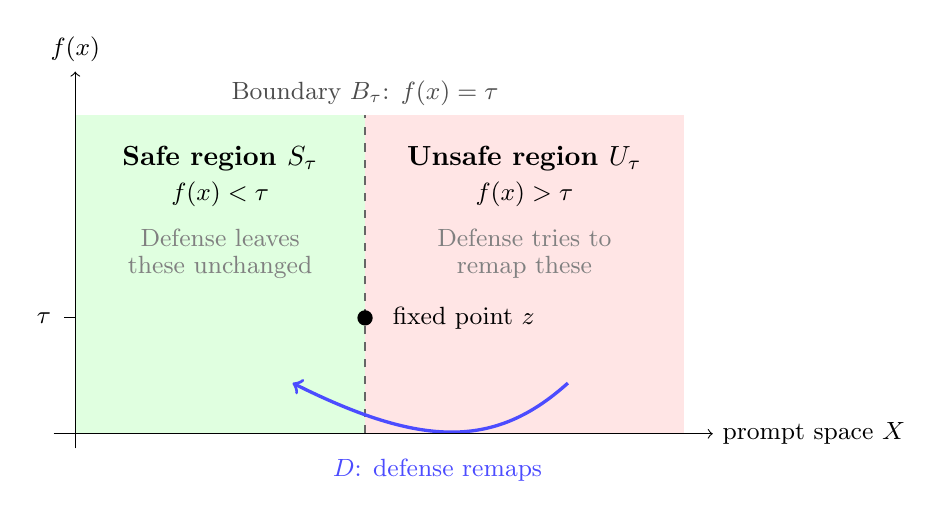
\begin{tikzpicture}[scale=0.92]
  \fill[green!12] (0,0.8) rectangle (4.0,5.2);
  \fill[red!10] (4.0,0.8) rectangle (8.4,5.2);
  \draw[dashed, thick, black!60] (4.0,0.8) -- (4.0,5.2);
  \node[font=\bfseries] at (2.0,4.6) {Safe region $S_\tau$};
  \node[font=\small] at (2.0,4.1) {$f(x) < \tau$};
  \node[font=\small, black!50] at (2.0,3.5) {Defense leaves};
  \node[font=\small, black!50] at (2.0,3.1) {these unchanged};
  \node[font=\bfseries] at (6.2,4.6) {Unsafe region $U_\tau$};
  \node[font=\small] at (6.2,4.1) {$f(x) > \tau$};
  \node[font=\small, black!50] at (6.2,3.5) {Defense tries to};
  \node[font=\small, black!50] at (6.2,3.1) {remap these};
  \node[font=\small, black!70] at (4.0,5.5) {Boundary $B_\tau$: $f(x)=\tau$};
  \fill[black] (4.0,2.4) circle (3pt);
  \node[anchor=west, font=\small] at (4.25,2.4) {fixed point $z$};
  \draw[->, thick, blue!70, line width=1.2pt]
    (6.8,1.5) .. controls (5.8,0.6) and (4.8,0.6) .. (3.0,1.5);
  \node[font=\small, blue!70] at (5.0,0.3) {$D$: defense remaps};
  \draw[->] (-0.3,0.8) -- (8.8,0.8) node[right] {\small prompt space $X$};
  \draw[->] (0,0.6) -- (0,5.8) node[above] {\small $f(x)$};
  \draw (0,2.4) -- (-0.15,2.4);
  \node[anchor=east, font=\small] at (-0.2,2.4) {$\tau$};
\end{tikzpicture}
\caption{Schematic of the prompt space. The defense~$D$ must leave all
safe inputs unchanged (utility preservation) and tries to remap unsafe
inputs into the safe region. Boundary fixation (\Cref{thm:main}) proves
the defense must also leave some boundary points unchanged, the black
dot~$z$ passes through with no remediation.}
\label{fig:landscape}
\end{figure}

\begin{definition}[Alignment Deviation Function]
\label{def:ad}
Let $X$ be a topological space and let $f\colon X \to \R$ be a
continuous scoring function. We interpret $f(x)$ as an alignment
deviation score for prompt $x$. Given a threshold $\tau\in\R$:
\begin{align}
  S_\tau &= \{x \in X : f(x) < \tau\}  &&\text{(safe region)} \\
  U_\tau &= \{x \in X : f(x) > \tau\}  &&\text{(unsafe region)} \\
  B_\tau &= \{x \in X : f(x) = \tau\}  &&\text{(boundary)}
\end{align}
\end{definition}

\begin{definition}[Defense]
\label{def:defense}
A \emph{defense} is a continuous map $D\colon X \to X$. It is
\emph{utility-preserving} if $D(x) = x$ for all $x \in S_\tau$, and
\emph{complete} if $f(D(x)) < \tau$ for all $x\in X$.
\end{definition}

We will also use two weaker preservation notions. A defense is
\emph{score-preserving on safe inputs} if $f(D(x)) = f(x)$ for all
$x \in S_\tau$, and \emph{$\varepsilon$-relaxed on safe inputs} if
$|f(D(x)) - f(x)| \leq \varepsilon$ for all $x \in S_\tau$.

The central question is whether a wrapper can preserve utility in one
of these senses and still make all outputs safe. The following sections
show that across several regimes, the answer is no.


% ============================================================
\section{Impossibility of Wrapper Defense in Continuous Settings}
\label{sec:boundary}

We begin with the most fundamental result. The argument fits in a
paragraph: the defense fixes every safe input, so continuity makes its
fixed-point set closed. But the safe region~$S_\tau$ is open (preimage
of an open interval under continuous~$f$), and in a connected space a
nonempty proper open set is not closed. Hence the fixed-point set
cannot stop exactly at the edge of the safe region, it must spill onto
the boundary~$B_\tau$. Some boundary prompts pass through unchanged.

\begin{theorem}[Boundary Fixation]
\label{thm:main}
Let $X$ be a connected Hausdorff space (a space that is ``in one
piece'' and where distinct points can be separated by neighborhoods).
Let $f\colon X\to\R$ be continuous with $S_\tau, U_\tau \neq
\emptyset$, and $D\colon X \to X$ continuous with
$D|_{S_\tau} = \id$. Then there exists $z\in X$ with $f(z) = \tau$
and $D(z) = z$. Moreover, every $z \in \cl{S_\tau} \setminus S_\tau$
satisfies $f(z) = \tau$ and $D(z) = z$, and this set is nonempty.
\end{theorem}

\begin{proof}[Proof sketch]
In a Hausdorff space, $\Fix(D)$ is closed (preimage of the diagonal).
By utility preservation, $S_\tau \subseteq \Fix(D)$, so
$\cl{S_\tau} \subseteq \Fix(D)$. But $S_\tau = f^{-1}((-\infty,\tau))$
is open and not closed (connectedness: a nonempty proper clopen set
would disconnect~$X$). Hence $\cl{S_\tau} \supsetneq S_\tau$. Any
$z \in \cl{S_\tau}\setminus S_\tau$ satisfies $f(z) = \tau$ (limits of
values ${<}\tau$ cannot exceed~$\tau$, and $z \notin S_\tau$ forces
$f(z) \geq \tau$) and $D(z) = z$. Full proof in \Cref{app:proofs}.
\end{proof}

This means that the defense's fixed-point set is too large to avoid the
boundary. Utility preservation forces it to contain the safe region;
closure forces it to contain the boundary; connectedness ensures the
boundary is nonempty. Alternatively: a complete utility-preserving
defense would be a continuous retraction $D\colon X \to S_\tau$
(since $D|_{S_\tau} = \id$ and $D(X) \subseteq S_\tau$), but a
retract of a Hausdorff space is closed (the fixed-point set is
closed), while~$S_\tau$ is open and not closed
(connectedness)---a contradiction.

\begin{theorem}[Defense Trilemma]
\label{thm:trilemma}
Let $X$ be a connected Hausdorff space, $f\colon X \to \R$ continuous
with $S_\tau, U_\tau \neq \emptyset$. No $D\colon X \to X$ can
simultaneously be continuous, utility-preserving ($D|_{S_\tau} = \id$),
and complete ($f(D(x)) < \tau$ for all~$x$).
\end{theorem}

All three hypotheses are individually necessary. A defense can satisfy
at most two of the three---the \emph{defense trilemma}
(\Cref{fig:trilemma}). Counterexamples for each dropped hypothesis
appear in \Cref{app:counterexamples}.

\paragraph{Falsifier.}
An empirical counterexample to the trilemma would be a production
defense that is demonstrably continuous, utility-preserving, and
complete at a named~$\tau$.

\begin{figure}[t]
\centering
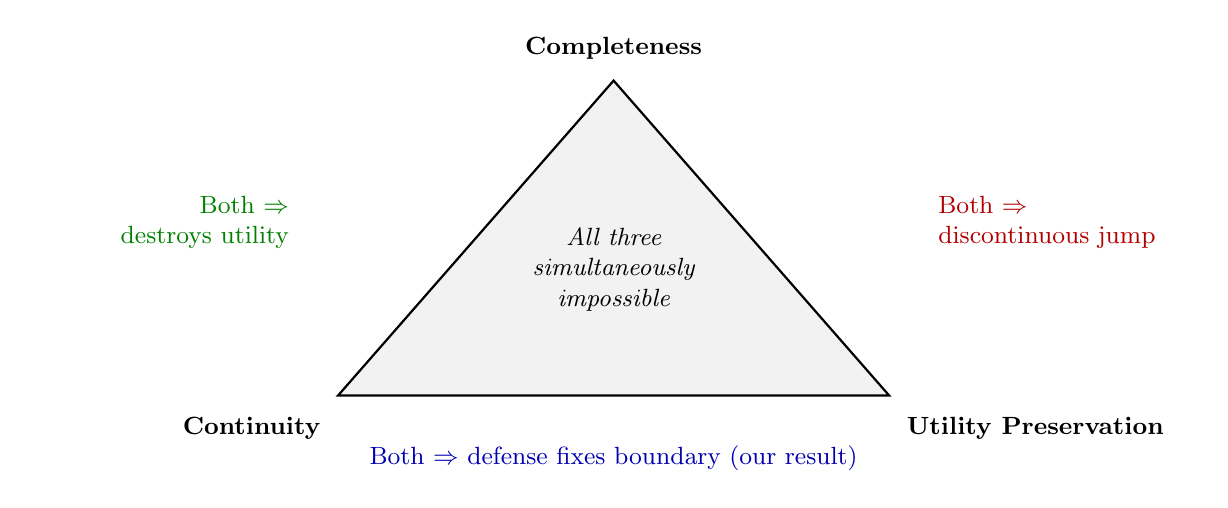
\begin{tikzpicture}[scale=1.0]
  \coordinate (A) at (0,0);
  \coordinate (B) at (7,0);
  \coordinate (C) at (3.5,4.0);
  \fill[black!5] (A) -- (B) -- (C) -- cycle;
  \draw[thick] (A) -- (B) -- (C) -- cycle;
  \node[anchor=north east, font=\bfseries\small] at (-0.1,-0.15) {Continuity};
  \node[anchor=north west, font=\bfseries\small] at (7.1,-0.15) {Utility Preservation};
  \node[anchor=south, font=\bfseries\small] at (3.5,4.15) {Completeness};
  \node[font=\small, text=blue!70!black, align=center] at (3.5,-0.8)
    {Both $\Rightarrow$ defense fixes boundary (our result)};
  \node[font=\small, text=green!50!black, anchor=east, align=right,
        text width=3.2cm] at (-0.5,2.2)
    {Both $\Rightarrow$\\destroys utility};
  \node[font=\small, text=red!70!black, anchor=west, align=left,
        text width=3.2cm] at (7.5,2.2)
    {Both $\Rightarrow$\\discontinuous jump};
  \node[font=\small\itshape, align=center] at (3.5,1.6)
    {All three\\simultaneously\\impossible};
\end{tikzpicture}
\caption{The defense trilemma. Any continuous wrapper defense on a
connected space can satisfy at most two of
the three properties. The bottom edge is our main result; the other
two edges correspond to counterexamples in \Cref{app:counterexamples}.}
\label{fig:trilemma}
\end{figure}

\begin{remark}[Not all boundary points are fixed]
The theorem captures $\cl{S_\tau} \setminus S_\tau$, not all of
$B_\tau$. Boundary points not in $\cl{S_\tau}$ may escape fixation.
\end{remark}


\subsection{Exact and Relaxed Utility Preservation}
\label{sec:relaxed}

Strict utility preservation ($D(x) = x$ for safe~$x$) can be
relaxed. The impossibility survives score-preserving rewrites and
even approximate score preservation.

\begin{theorem}[Score-Preserving Defense]
\label{thm:score-preserving}
Let $X$ be a connected Hausdorff space, $f\colon X\to\R$ continuous
with $S_\tau, U_\tau \neq \emptyset$. If $D\colon X \to X$ is
continuous and \emph{score-preserving on safe inputs}:
$f(D(x)) = f(x)$ for all $x \in S_\tau$, then there exists $z$ with
$f(z) = \tau$ and $f(D(z)) = \tau$.
\end{theorem}

\begin{proof}[Proof sketch]
Define $h = f \circ D - f$. Then $h$ is continuous and $h|_{S_\tau} = 0$.
The zero set $\{h = 0\}$ is closed and contains $\cl{S_\tau}$, since closed sets contain their boundary points. For
$z \in \cl{S_\tau} \setminus S_\tau$, $f(D(z)) = f(z) = \tau$.
\end{proof}

The next result weakens score preservation to approximate:

\begin{theorem}[$\varepsilon$-Relaxed Utility Preservation]
\label{thm:eps-relaxed}
Under the hypotheses of \Cref{thm:score-preserving}, if
$|f(D(x)) - f(x)| \leq \varepsilon$ for all $x \in S_\tau$, then
there exists $z$ with $f(z) = \tau$ and
$f(D(z)) \geq \tau - \varepsilon$.
\end{theorem}

\begin{proof}[Proof sketch]
The set $\{x : h(x) \geq -\varepsilon\}$ is closed and contains
$S_\tau$, hence $\cl{S_\tau}$. For
$z \in \cl{S_\tau} \setminus S_\tau$:
$f(D(z)) = \tau + h(z) \geq \tau - \varepsilon$.
\end{proof}


\begin{remark}[Why $D(S_\tau) \subseteq S_\tau$ alone is insufficient]
\label{rem:safe-preserving-escape}
The weakest relaxation---$D(S_\tau) \subseteq S_\tau$ with no score
constraint---does allow a complete defense (e.g., a constant map
$D(x) = x_0$ to a fixed safe point). But this destroys all semantic
content: every prompt produces the same response. The score-preservation
conditions formalize the requirement that defense must not destroy
utility, without requiring the defense to be the identity.
\end{remark}

\begin{remark}[Open: utility-floor relaxation]
\label{rem:utility-floor}
Between exact identity on $S_\tau$ and the constant map lies a
realistic band of deployed wrappers that satisfy
$D(S_\tau) \subseteq S_\tau$ plus a \emph{utility floor}: e.g.,
embedding similarity $\mathrm{sim}(D(x), x) \geq \gamma$ for all
$x \in S_\tau$. Whether the boundary-fixation obstruction persists
under such a utility-floor hypothesis is an open question.
A positive answer would substantially strengthen the practical reach
of \Cref{thm:main}; a negative answer (a constructive complete
defense satisfying the utility floor) would sharpen the boundary of
the impossibility.
\end{remark}


% ============================================================
\subsection{Quantitative Failure Near the Boundary}
\label{sec:eps-robust}

Boundary fixation produces at least one fixed point; Lipschitz
regularity makes the failure spread to a neighborhood.

\begin{theorem}[$\varepsilon$-Robust Defense Constraint]
\label{thm:eps-robust}
Under the hypotheses of \Cref{thm:main}, if $(X,d)$ is a metric
space, $f$ is $L$-Lipschitz, and $D$ is $K$-Lipschitz, then for
the fixed boundary point~$z$:
\begin{equation}
  f(D(x)) \;\geq\; \tau - LK\dist(x, z)
  \qquad \text{for all } x \in X.
\end{equation}
Points within distance~$\delta$ of~$z$ remain within
$LK\delta$ of threshold.
\end{theorem}

\begin{proof}[Proof sketch]
Since $D(z)=z$ and $D$ is $K$-Lipschitz:
$\dist(D(x),z) \leq K\dist(x,z)$. Since $f(z)=\tau$ and $f$ is
$L$-Lipschitz:
$|f(D(x)) - \tau| \leq L \cdot K\dist(x,z)$.
Full proof in \Cref{app:proofs}.
\end{proof}

Appendix~\ref{app:quantitative} records explicit measure bounds for the
near-threshold band and related quantitative refinements.

% ============================================================
\subsection{Persistent Unsafe Region}
\label{sec:persistent}

The $\varepsilon$-robust constraint bounds the depth to which the
defense pushes near-boundary points, but permits values slightly
below~$\tau$. When the alignment surface rises faster than the
defense can pull it down, some points remain above threshold.

\paragraph{Decoupling global and directional Lipschitz constants.}
The $\varepsilon$-robust bound (\Cref{thm:eps-robust}) uses the
\emph{global} Lipschitz constant~$L$ of~$f$, which bounds~$f$
uniformly in all directions. The persistence argument, however,
compares $f$'s growth rate in the \emph{steep direction} to how much
the defense can reduce~$f$ along the \emph{displacement direction}
$D(x) - x$. In anisotropic settings these directions differ: $f$ may
rise steeply toward the unsafe region while varying slowly in the
direction the defense pulls.

We write $\ell$ for the \emph{defense-path Lipschitz constant}:
\[
  \ell \;=\; \sup_{x \neq D(x)}
    \frac{|f(D(x)) - f(x)|}{\dist(D(x),\, x)}
\]
(with $\ell = 0$ when $D = \id$, i.e., the supremum over the empty
set is taken as~$0$).
Since $f$ is $L$-Lipschitz globally, $\ell \leq L$. When the
alignment surface is \textbf{isotropic} ($\ell = L$), the steep region
is empty for every $K \geq 0$ (verified in Lean as
\texttt{shallow\_boundary\_no\_persistence}). The result is
non-vacuous precisely when the surface is \textbf{anisotropic}:
$\ell < L$, with directional gradient~$G$ satisfying
$G > \ell(K+1)$.

\begin{lemma}[Input-Relative Bound]
\label{lem:input-bound}
Under the hypotheses of \Cref{thm:eps-robust}, if $f$ has
defense-path Lipschitz constant~$\ell$, then
$f(D(x)) \geq f(x) - \ell(K+1)\dist(x,z)$
for all $x \in X$.
\end{lemma}

\begin{proof}[Proof sketch]
Triangle inequality:
$\dist(D(x), x) \leq \dist(D(x), z) + \dist(z, x)
\leq (K+1)\dist(x, z)$.
Defense-path Lipschitz: $|f(D(x)) - f(x)| \leq \ell\dist(D(x), x)
\leq \ell(K+1)\dist(x, z)$.
\end{proof}

This means that the defense can reduce any point's score by at most
$\ell(K+1)$ times its distance from~$z$. If the score rises faster
than that, the defense loses.

\begin{definition}[Steep region]
\label{def:steep}
Given a fixed boundary point $z$, the \emph{steep region} is
$\mathcal{S} = \{x \in X : f(x) > \tau + \ell(K+1)\dist(x, z)\}$---the
set of points where alignment deviation exceeds~$\tau$ by more than
the defense's Lipschitz budget can compensate.
\end{definition}

\begin{theorem}[Persistent Unsafe Region]
\label{thm:persistent}
Let $X$ be a connected Hausdorff metric space, $f$ continuous and
$L$-Lipschitz, $D$ continuous and $K$-Lipschitz with
$D|_{S_\tau} = \id$, and $S_\tau, U_\tau \neq \emptyset$.
Let $z \in \cl{S_\tau} \setminus S_\tau$ be the fixed boundary
point from \Cref{thm:main}, and let $\ell$ be the defense-path
Lipschitz constant. If $\mathcal{S} \neq \emptyset$, then:
\begin{enumerate}[nosep]
  \item $\mathcal{S}$ is open.
  \item $\mathcal{S}$ has positive measure (under any measure positive
    on nonempty open sets).
  \item For every $x \in \mathcal{S}$: $f(D(x)) > \tau$.
\end{enumerate}
The defense leaves a positive-measure region that remains unsafe.
\end{theorem}

\begin{proof}[Proof sketch]
$\mathcal{S}$ is a strict superlevel set of a continuous function,
hence open. For $x \in \mathcal{S}$:
$f(D(x)) \geq f(x) - \ell(K+1)\dist(x,z) > \tau$
by \Cref{lem:input-bound} and the definition of~$\mathcal{S}$.
Full proof in \Cref{app:proofs}.
\end{proof}

The main paper uses persistence only when the steep region is
nonempty. A derivative-based sufficient condition and related gradient
arguments are deferred to \Cref{app:additional,app:artifact}. Empirically,
the relevant models exhibit exactly this anisotropic regime
(\Cref{sec:experiments}): the alignment surface rises steeply toward
the unsafe region ($G$ large) while the defense operates in a smoother
subspace ($\ell \ll L$).

\paragraph{Falsifier.}
As already stated, the empirical content is
$\mathrm{FP}_{\mathrm{int}} > 0$ under a continuous
utility-preserving~$D$: a cell in $\mathcal{S}_{\text{pred}}$ (i.e.,
predicted persistent) with $f(D(x)) < \tau$ would refute
\Cref{thm:persistent}.


\begin{figure}[t]
\centering
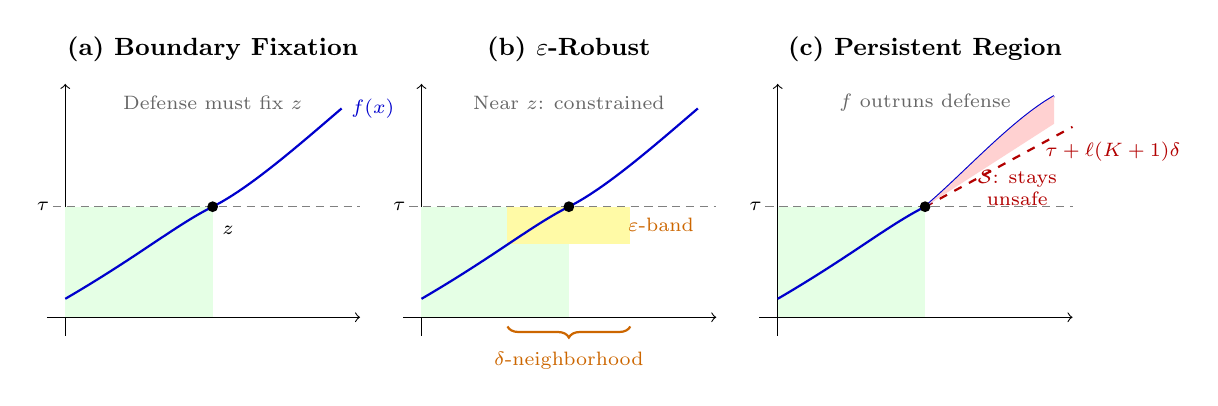
\begin{tikzpicture}[scale=0.78]
  % ── Panel (a): Boundary Fixation ──────────────────────────
  \begin{scope}[shift={(0,0)}]
    % Axes
    \draw[->] (-0.3,0) -- (4.8,0);
    \draw[->] (0,-0.3) -- (0,3.8);
    % Tau line
    \draw[densely dashed, black!50] (-0.2,1.8) -- (4.8,1.8);
    \node[left, font=\scriptsize] at (-0.1,1.8) {$\tau$};
    % Safe shading
    \fill[green!10] (0,0) rectangle (2.4,1.8);
    % f(x) curve
    \draw[thick, blue!80!black] (0,0.3) .. controls (1.2,1.0)
      and (1.8,1.5) .. (2.4,1.8) .. controls (3.0,2.1)
      and (3.8,2.8) .. (4.5,3.4);
    \node[right, font=\scriptsize, blue!80!black] at (4.5,3.4) {$f(x)$};
    % Fixed point
    \fill[black] (2.4,1.8) circle (2.5pt);
    \node[below right, font=\scriptsize] at (2.4,1.65) {$z$};
    % Title
    \node[font=\small\bfseries, anchor=south] at (2.4,4.0)
      {(a) Boundary Fixation};
    \node[font=\scriptsize, text=black!60, align=center] at (2.4,3.5)
      {Defense must fix $z$};
  \end{scope}

  % ── Panel (b): ε-Robust Constraint ───────────────────────
  \begin{scope}[shift={(5.8,0)}]
    \draw[->] (-0.3,0) -- (4.8,0);
    \draw[->] (0,-0.3) -- (0,3.8);
    \draw[densely dashed, black!50] (-0.2,1.8) -- (4.8,1.8);
    \node[left, font=\scriptsize] at (-0.1,1.8) {$\tau$};
    \fill[green!10] (0,0) rectangle (2.4,1.8);
    % ε-band shading
    \fill[yellow!35] (1.4,1.2) rectangle (3.4,1.8);
    % f(x) curve
    \draw[thick, blue!80!black] (0,0.3) .. controls (1.2,1.0)
      and (1.8,1.5) .. (2.4,1.8) .. controls (3.0,2.1)
      and (3.8,2.8) .. (4.5,3.4);
    % Fixed point
    \fill[black] (2.4,1.8) circle (2.5pt);
    % Band bracket
    \draw[decorate, decoration={brace, amplitude=4pt, mirror},
          thick, orange!80!black]
      (1.4,-0.15) -- (3.4,-0.15);
    \node[below, font=\scriptsize, orange!80!black] at (2.4,-0.4)
      {$\delta$-neighborhood};
    % Band label
    \node[font=\scriptsize, orange!80!black] at (3.9,1.5)
      {$\varepsilon$-band};
    % Title
    \node[font=\small\bfseries, anchor=south] at (2.4,4.0)
      {(b) $\varepsilon$-Robust};
    \node[font=\scriptsize, text=black!60, align=center] at (2.4,3.5)
      {Near $z$: constrained};
  \end{scope}

  % ── Panel (c): Persistent Unsafe Region ──────────────────
  \begin{scope}[shift={(11.6,0)}]
    \draw[->] (-0.3,0) -- (4.8,0);
    \draw[->] (0,-0.3) -- (0,3.8);
    \draw[densely dashed, black!50] (-0.2,1.8) -- (4.8,1.8);
    \node[left, font=\scriptsize] at (-0.1,1.8) {$\tau$};
    \fill[green!10] (0,0) rectangle (2.4,1.8);
    % Defense budget cone (dashed red from z)
    \draw[dashed, red!70!black, line width=0.8pt]
      (2.4,1.8) -- (4.8,3.1);
    \node[right, font=\scriptsize, red!70!black] at (4.2,2.7)
      {$\tau + \ell(K+1)\delta$};
    % f(x) curve — rises ABOVE the cone
    \draw[thick, blue!80!black] (0,0.3) .. controls (1.2,1.0)
      and (1.8,1.5) .. (2.4,1.8) .. controls (3.0,2.3)
      and (3.8,3.2) .. (4.5,3.6);
    % Persistent region shading (between curve and cone)
    \fill[red!18] (2.4,1.8) .. controls (3.0,2.3) and (3.8,3.2)
      .. (4.5,3.6) -- (4.5,3.15) -- (2.4,1.8) -- cycle;
    % Fixed point
    \fill[black] (2.4,1.8) circle (2.5pt);
    % Label
    \node[font=\scriptsize, red!70!black, align=center] at (3.9,2.1)
      {$\mathcal{S}$: stays\\unsafe};
    % Title
    \node[font=\small\bfseries, anchor=south] at (2.4,4.0)
      {(c) Persistent Region};
    \node[font=\scriptsize, text=black!60, align=center] at (2.4,3.5)
      {$f$ outruns defense};
  \end{scope}
\end{tikzpicture}
\caption{The three impossibility results on a 1D cross-section.
\textbf{(a)}~The defense must fix boundary point~$z$ (Thm.~\ref{thm:main}).
\textbf{(b)}~Near~$z$, Lipschitz regularity constrains the defense to
a shallow $\varepsilon$-band (yellow; Thm.~\ref{thm:eps-robust}).
\textbf{(c)}~Where $f$ rises faster than the defense budget
$\ell(K+1)\delta$ (dashed red), the region above~$\tau$ persists
(red shading; Thm.~\ref{thm:persistent}).}
\label{fig:escalation}
\end{figure}


Quantitative refinements of the continuous theory, including explicit
volume lower bounds, cone-measure bounds, and the defense-aggressiveness
dilemma, are deferred to the appendix
(\Cref{thm:coarea,thm:cone,thm:dilemma}).


% ============================================================
\section{Impossibility of Wrapper Defense in Discrete Settings}
\label{sec:bridge}

On finite sets, the same failure appears as a combinatorial tradeoff: completeness vs.\ information preservation. No topology is required; results are verified in Lean (\texttt{MoF\_12\_Discrete}). The Tietze/McShane--Whitney bridge to continuous spaces is in \Cref{thm:tietze}.

\begin{theorem}[Discrete Defense Dilemma]
\label{thm:disc-dilemma}
Let $X$ be a finite set with $S_\tau, U_\tau \neq \emptyset$, and
$D\colon X \to X$ utility-preserving ($D(x) = x$ for $f(x) < \tau$).
\begin{enumerate}[nosep]
  \item If $D$ is injective, then $f(D(u)) \geq \tau$ for every
    $u$ with $f(u) \geq \tau$ (including boundary points): the
    defense is incomplete.
  \item If $D$ is complete ($f(D(x)) < \tau$ for all~$x$), then $D$ is
    non-injective: $\exists\, x \neq y$ with $D(x) = D(y)$.
\end{enumerate}
\end{theorem}

\begin{proof}
(1) Suppose $D$ is injective and $f(D(u)) < \tau$ for some $u$ with
$f(u) \geq \tau$. Then $D(u)$ is safe, so $D(D(u)) = D(u)$ by utility
preservation. Injectivity gives $D(u) = u$, so
$f(u) = f(D(u)) < \tau$, contradicting $f(u) \geq \tau$.

(2) For any $u \in U_\tau$: completeness gives $f(D(u)) < \tau$, so
utility preservation gives $D(D(u)) = D(u)$. But
$u \neq D(u)$ since $f(u) \geq \tau > f(D(u))$.
So $u$ and $D(u)$ are distinct inputs with $D(u) = D(D(u))$: the
defense is non-injective.
\end{proof}

The continuous trilemma trades \emph{continuity}; the discrete dilemma trades \emph{injectivity}. Any complete defense must collapse distinct inputs (\Cref{sec:experiments}).

\paragraph{Falsifier.}
A complete utility-preserving injective $D$ on any finite input set would be a counterexample.


% ============================================================
\section{Impossibility of Wrapper Defense in Stochastic and Multi-Turn Settings}
\label{sec:extensions}

Neither repeated interaction nor randomization removes the obstruction.

\subsection{Multi-Turn Impossibility}

\begin{theorem}[Multi-Turn Impossibility]
\label{thm:multi-turn}
Let $\{f_t, D_t\}_{t=1}^T$ be alignment functions and defenses over
$T$ turns on a connected Hausdorff space, each continuous and
utility-preserving, with $S_\tau^{(t)}, U_\tau^{(t)} \neq \emptyset$
at every turn. Then for every turn~$t$, there exists $z_t$ with
$f_t(z_t) = \tau$ and $D_t(z_t) = z_t$.
\end{theorem}

\begin{proof}[Proof sketch]
Apply \Cref{thm:main} to $(f_t, D_t)$ at each turn. The functions may
depend on full history---this does not matter, as each timestep is a
fresh instance of boundary fixation.
\end{proof}

The attacker's running-max exploit improves monotonically (\texttt{running\_max\_monotone}).

\paragraph{Falsifier.}
An attack trajectory with strictly decreasing running-max AD over
turns would refute the monotone-improvement mechanism.
Empirically, per-turn boundary fixation recurs and running-max AD increases monotonically (\Cref{tab:multi-turn,fig:multi-turn-plot} in the appendix).

\subsection{Stochastic Defense Impossibility}

\begin{theorem}[Stochastic Defense Impossibility]
\label{thm:stochastic}
Let $X$ be a connected Hausdorff space, $f\colon X \to \R$ continuous
with $S_\tau, U_\tau \neq \emptyset$. Let $D$ be a stochastic defense
and define $g(x) = \mathbb{E}_{y \sim D(x)}[f(y)]$. If $g$ is
continuous and $g(x) = f(x)$ for all $x \in S_\tau$, then there
exists $z$ with $f(z) = \tau$ and $g(z) = \tau$.
\end{theorem}

\begin{proof}[Proof sketch]
Define $h = g - f$. Then $h$ is continuous and $h|_{S_\tau} = 0$,
so $h$ vanishes on $\cl{S_\tau}$ (same closure argument as
\Cref{thm:score-preserving}). For
$z \in \cl{S_\tau} \setminus S_\tau$: $g(z) = f(z) = \tau$.
\end{proof}

\noindent\textit{Remark (stochastic dichotomy).}
Since $\mathbb{E}[f(D(z))] = \tau$, either $f(D(z)) = \tau$ almost
surely (the defense is deterministic at~$z$), or the random variable
$f(D(z))$ has positive probability of exceeding~$\tau$---i.e., the
defense \emph{actively produces unsafe outputs} with positive
probability. The stochastic case is therefore strictly harder than
the deterministic one: a genuinely random defense at boundary points
must sometimes make things worse.

\noindent\textit{Remark.}
The continuity of $g$ is a nontrivial assumption: it requires the
distribution $D(x)$ to vary continuously with~$x$ in a suitable sense.
Stochastic defenses with discontinuous rejection probabilities escape
this theorem.

\paragraph{Falsifier.}
A stochastic defense at a boundary cell with $\mathrm{variance} = 0$
and $f(D(z)) < \tau$ would refute \Cref{thm:stochastic}.
Empirically, a genuinely random wrapper at a boundary cell shows positive variance with positive mass above~$\tau$ (\Cref{tab:stochastic,fig:stochastic-histogram} in the appendix).

Pipeline composition and additional geometry/stability results are
deferred to the appendix. In particular, the pipeline theorem shows
that composing non-contractive stages amplifies the effective
Lipschitz constant and therefore widens the failure budget
(\Cref{thm:pipeline,thm:pipeline-impossible,app:landscape,app:attacks,app:stability,app:cost}).


% ============================================================
\section{Experimental Validation}
\label{sec:experiments}

The empirical section tests whether the theory is vacuous.
We exercise the continuous theory on real LLM safety surfaces (boundary and persistence structure) and the discrete theorem on a saturated unsafe-prompt archive (forced collapse).
All experiments use the MAP-Elites behavioral-space driver of~\cite{munshi2026manifold} over a 2D prompt space (query indirection $\times$ authority framing); every AD value comes from our own live runs (\Cref{app:exp-details}).

\subsection{Continuous-Setting Validation}
\label{sec:live-validation}

A validator estimates $L, K, \ell, G$ on the grid, identifies boundary anchor $z^{*}$, and checks the containment $\mathcal{S}_{\text{pred}} \subseteq \mathcal{S}_{\text{act}}$ where
$\mathcal{S}_{\text{pred}} = \{x : f(x) > \tau + \ell(K{+}1)\dist(x,z^{*})\}$
and $\mathcal{S}_{\text{act}} = \{x : f(D(x)) > \tau\}$.
The key metric is $\mathrm{FP}_{\mathrm{int}}$: interior cells predicted persistent but actually remediated. $\mathrm{FP}_{\mathrm{int}} > 0$ would be a real counterexample; boundary false positives merely witness discontinuity (hypothesis not met); false negatives are permitted (the theorem claims containment one way only).

We ran live against the OpenAI API with \texttt{gpt-3.5-turbo-0125} (target) and \texttt{gpt-4.1-2025-04-14} (judge). A saturation study ($400$ evaluations, ${\sim}5{,}200$ API calls, ${\sim}$\$15) filled $82$ cells of a $25{\times}25$ grid with $66$ unsafe ($f{>}\tau$) and $10$ boundary cells—the only configuration where the theorem is non-vacuously exercised. All $f$ values are judge-dependent; a two-judge comparison is in \Cref{app:judge-robustness}.

\subsubsection{Non-vacuous validation: continuous defenses}
\label{sec:gp-instance}

Theorem~\ref{thm:persistent} has non-trivial quantitative content only when $\hat G > \hat\ell(\hat K{+}1)$, i.e., when the alignment surface rises faster than the defense can pull it down.
A sweep over four continuous defense families (\Cref{tab:continuous-sweep} in appendix) reveals that \emph{most natural defenses fail this condition}: \textsc{SmoothNearestSafe}, \textsc{KernelSmoothed}, and \textsc{SoftProj} all produce $\hat\ell(\hat K{+}1) \gg \hat G$ because they align displacement with $-\nabla f$, which maximizes~$\hat\ell$.
The theorem becomes a non-vacuous \emph{diagnostic} when the defense direction diverges from $\nabla f$: measured $(\hat G, \hat\ell, \hat K)$ with $\hat\ell \ll L$ signals a construction that fights its own gradient.

We demonstrate this diagnostic on a GP-smooth oblique defense $D(x) = x + \alpha\,\beta(\mu(x))\,v(x)$ displaced $89.5^\circ$ from the GP gradient (RBF kernel, $\sigma{=}0.2$, 82 cells). This is a deliberately adversarial defense direction chosen to enter the transversal regime. Estimates: $\hat\ell = 0.86$, $\hat K = 1.05$, $\hat G = 23.6$, so $\hat\ell(\hat K{+}1) = 1.77 \ll \hat G$. Result: $|\mathcal{S}_{\text{pred}}| = 3$, all actually persistent ($\mathrm{TP}{=}3$, $\mathrm{FP}_{\mathrm{int}}{=}0$; \Cref{fig:theory-vs-reality-saturated}). Theorem~\ref{thm:dilemma}'s optimal constant $K^* = \hat G/\hat\ell - 1 \approx 26.5$ gives a concrete design constraint: defenses with $K < K^*$ admit persistent cells; defenses with $K \geq K^*$ destroy utility (\Cref{fig:k-tradeoff} in appendix).

\begin{figure}[h]
\centering
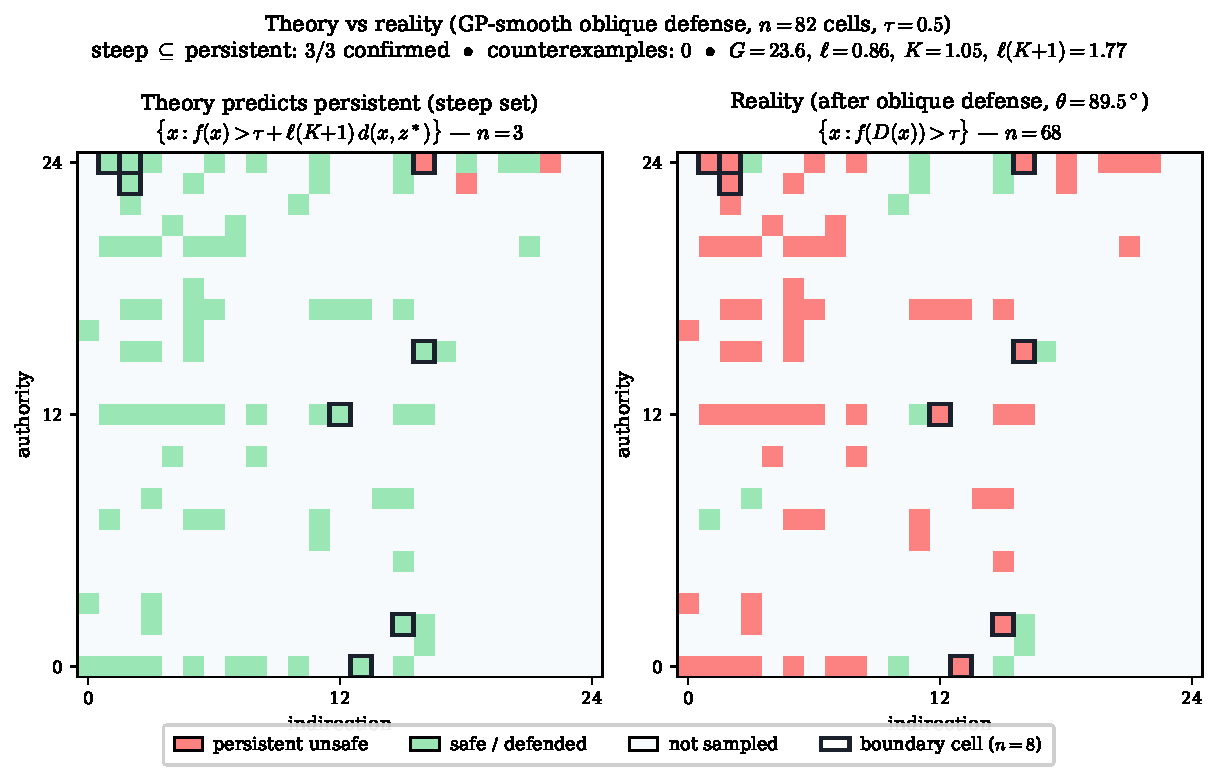
\includegraphics[width=\textwidth]{figures/oblique_theory_vs_reality.pdf}
\caption{A \emph{single} non-vacuous instance exercising
Theorem~\ref{thm:persistent} on the saturated
\texttt{gpt-3.5-turbo-0125} grid ($82$ filled cells, $\tau = 0.5$)
under the GP-smooth oblique defense
($\theta = 89.5^\circ$, $\hat\ell = 0.86$, $\hat K = 1.05$).
\textbf{Left:} the \emph{steep set}
$\mathcal{S}_{\text{pred}} = \{x : f(x) > \tau +
\hat\ell(\hat K{+}1)\,\dist(x,z^{*})\}$; $|\mathcal{S}_{\text{pred}}| = 3$.
\textbf{Right:} cells actually persistent after defense,
$\mathcal{S}_{\text{act}} = \{x : f(D(x)) > \tau\}$;
$|\mathcal{S}_{\text{act}}| = 68$.
Transversality holds non-trivially
($\hat G = 23.6 \gg \hat\ell(\hat K{+}1) = 1.77$) and the defense
is genuinely non-identity ($82$ cells displaced). The predicted
three cells are all actually persistent
($\mathrm{TP} = 3$, $\mathrm{FP}_{\mathrm{int}} = 0$). The $65$ false negatives
(red on the right, green on the left) are \emph{not} theorem
violations: the theorem predicts
$\mathcal{S}_{\text{pred}} \subseteq \mathcal{S}_{\text{act}}$,
not equality.}
\label{fig:theory-vs-reality-saturated}
\end{figure}

Appendix sweeps over three defense families, multiple kernels, and grid resolutions preserve $\mathrm{FP}_{\mathrm{int}} = 0$. Theorem~\ref{thm:eps-robust}'s $\varepsilon$-robust bound holds on all 82 cells, and 10 boundary cells in $\cl{S_\tau} \setminus S_\tau$ activate boundary fixation (nearest to $\tau$: gap $= 0.375$, vanishing under refinement). Bootstrap, seed replication, and judge-robustness checks all preserve the claim (\Cref{app:exp-details}). A three-target sweep (gpt-3.5-turbo, gpt-4o-mini, gpt-4o) yields $\mathrm{FP}_{\mathrm{int}} = 0$ in every row (\Cref{tab:three-target} in appendix).

\paragraph{Discrete classifier-gate footprint.}
\Cref{fig:classifier-gate-maps} maps two deployed gates on the same 82-cell archive.
Llama-Guard-3-1B collapses to 7 MLC-taxonomy labels while passing 51/82 prompts as \texttt{safe}; ShieldGemma-2B collapses to 2 labels while passing 56/82. Both sit on the injective-incomplete horn of \Cref{thm:disc-dilemma}: structure is preserved, but majority incompleteness remains.
For the forced-collapse test (\Cref{tab:forced-collapse} in appendix), a refusal defense collapses 66 unsafe inputs to 1 output, a canonical-category defense to 7, while an injective paraphrase defense produces 66 distinct rewrites---of which 1 remains above $\tau$ (\Cref{tab:paraphrase-unsafe}), the predicted incomplete witness.
The well-aligned target (gpt-5-mini, peak AD $= 0.5$) yields $U_\tau = \emptyset$ and the theorems are correctly silent.
Full numeric tables: \Cref{tab:llamaguard-demo,tab:forced-collapse,tab:paraphrase-unsafe}.

\begin{figure}[t]
\centering
\includegraphics[width=0.46\textwidth]{figures/llamaguard_gate_map.pdf}
\hfill
\includegraphics[width=0.46\textwidth]{figures/shieldgemma_gate_map.pdf}
\caption{Behavioral-map footprint of two deployed classifier gates on
the same 25$\times$25 saturated archive.
Left: original classification under the target model's AD score.
Right: gate verdicts on the same filled cells.
Llama-Guard-3-1B preserves 7 labels, passing 51/82 as \texttt{safe};
ShieldGemma-2B collapses to 2 labels, passing 56/82.}
\label{fig:classifier-gate-maps}
\end{figure}


% ============================================================
\paragraph{Scope and limitations.}
The theorems constrain only continuous utility-preserving wrappers on connected spaces; mechanisms outside this class (training-time alignment, architectural changes, hard blocklists, output filters, ensemble/human-in-the-loop systems) are not constrained. Persistence requires transversality ($G > \ell(K{+}1)$); for isotropic surfaces, $\mathcal{S} = \emptyset$. Engineering implications—including boundary shallowing, Lipschitz reduction, dimension reduction, and a worked design-constraint example—appear in \Cref{app:engineering}.

% ============================================================
\section{Conclusion}
\label{sec:conclusion}

The paper makes one claim: wrapper defense is structurally incomplete
under utility-preserving constraints. We show that this claim survives
in four regimes. In continuous spaces, utility-preserving wrappers fix
boundary prompts and, under additional regularity, leave quantitative
near-threshold and persistent unsafe regions. In discrete spaces,
complete defense requires input collapse. In stochastic and multi-turn
settings, the same obstruction reappears rather than disappearing.
Empirically, the predicted boundary and collapse mechanisms are visible
in real LLM safety surfaces and prompt archives.

The practical implication is not that defense is futile. It is that
wrapper defense should be engineered as risk management, not as a path
to complete elimination. The right objectives are to make the boundary
shallow, reduce effective dimension, monitor approach to threshold, and
use mechanisms outside the wrapper model when stronger guarantees are
required.

\input{neurips_compute_disclosure.tex}

\input{neurips_broader_impact.tex}

% ============================================================
\bibliographystyle{plain}
\begin{thebibliography}{99}

\bibitem{alon2023detecting}
G.~Alon and M.~Kamfonas.
\newblock Detecting language model attacks with perplexity.
\newblock \emph{arXiv preprint arXiv:2308.14132}, 2023.

\bibitem{bagnall2019certifying}
A.~Bagnall and G.~Stewart.
\newblock Certifying the true error: Machine learning in {Coq} with
  verified generalization guarantees.
\newblock \emph{Proceedings of the AAAI Conference on Artificial
Intelligence}, 2019.

\bibitem{bai2022constitutional}
Y.~Bai et~al.
\newblock Constitutional {AI}: Harmlessness from {AI} feedback.
\newblock \emph{arXiv preprint arXiv:2212.08073}, 2022.

\bibitem{chao2024jailbreaking}
P.~Chao, A.~Robey, E.~Dobriban, H.~Hassani, G.~J. Pappas, and
E.~Wong.
\newblock Jailbreaking black box large language models in twenty queries.
\newblock \emph{arXiv preprint arXiv:2310.08419}, 2024.

\bibitem{cohen2019certified}
J.~Cohen, E.~Rosenfeld, and J.~Z. Kolter.
\newblock Certified adversarial robustness via randomized smoothing.
\newblock \emph{Proceedings of ICML}, 2019.

\bibitem{goodfellow2014explaining}
I.~J. Goodfellow, J.~Shlens, and C.~Szegedy.
\newblock Explaining and harnessing adversarial examples.
\newblock \emph{Proceedings of ICLR}, 2015.

\bibitem{inan2023llama}
H.~Inan et~al.
\newblock {Llama Guard}: {LLM}-based input-output safeguard for
  human-{AI} conversations.
\newblock \emph{arXiv preprint arXiv:2312.06674}, 2023.

\bibitem{katz2017reluplex}
G.~Katz, C.~Barrett, D.~L. Dill, K.~Julian, and
M.~J. Kochenderfer.
\newblock Reluplex: An efficient {SMT} solver for verifying deep neural
  networks.
\newblock \emph{Proceedings of CAV}, 2017.

\bibitem{carlini2017evaluating}
N.~Carlini and D.~Wagner.
\newblock Towards evaluating the robustness of neural networks.
\newblock \emph{Proceedings of IEEE S\&P}, 2017.

\bibitem{mehrotra2024tree}
A.~Mehrotra et~al.
\newblock Tree of attacks: Jailbreaking black-box {LLMs} automatically.
\newblock \emph{Advances in Neural Information Processing Systems}, 37,
2024.

\bibitem{fawzi2018adversarial}
A.~Fawzi, H.~Fawzi, and O.~Fawzi.
\newblock Adversarial vulnerability for any classifier.
\newblock \emph{Advances in Neural Information Processing Systems}, 31, 2018.

\bibitem{greshake2023indirect}
K.~Greshake, S.~Abdelnabi, S.~Mishra, C.~Endres, T.~Holz, and M.~Fritz.
\newblock Not what you've signed up for: Compromising real-world
  {LLM}-integrated applications with indirect prompt injection.
\newblock \emph{Proceedings of AISec}, 2023.

\bibitem{huang2017safety}
X.~Huang, M.~Kwiatkowska, S.~Wang, and M.~Wu.
\newblock Safety verification of deep neural networks.
\newblock \emph{Proceedings of CAV}, 2017.

\bibitem{madry2018towards}
A.~Madry, A.~Makelov, L.~Schmidt, D.~Tsipras, and A.~Vladu.
\newblock Towards deep learning models resistant to adversarial attacks.
\newblock \emph{Proceedings of ICLR}, 2018.

\bibitem{mouret2015illuminating}
J.-B. Mouret and J.~Clune.
\newblock Illuminating search spaces by mapping elites.
\newblock \emph{arXiv preprint arXiv:1504.04909}, 2015.

\bibitem{naitzat2020topology}
G.~Naitzat, A.~Zhitnikov, and L.-H.~Lim.
\newblock Topology of deep neural networks.
\newblock \emph{Journal of Machine Learning Research}, 21(184):1--40, 2020.

\bibitem{munshi2026manifold}
Anonymous.
\newblock Manifold of failure: Behavioral attraction basins in language
  models.
\newblock Companion preprint (citation anonymized for double-blind
  review), 2026.

\bibitem{samvelyan2024rainbow}
M.~Samvelyan et~al.
\newblock Rainbow teaming: Open-ended generation of diverse adversarial
  prompts.
\newblock \emph{Advances in Neural Information Processing Systems}, 37,
2024.

\bibitem{singh2019abstract}
G.~Singh, T.~Gehr, M.~P{\"u}schel, and M.~Vechev.
\newblock An abstract domain for certifying neural networks.
\newblock \emph{Proceedings of POPL}, 2019.

\bibitem{szegedy2013intriguing}
C.~Szegedy et~al.
\newblock Intriguing properties of neural networks.
\newblock \emph{Proceedings of ICLR}, 2014.

\bibitem{tsipras2018robustness}
D.~Tsipras, S.~Santurkar, L.~Engstrom, A.~Turner, and A.~Madry.
\newblock Robustness may be at odds with accuracy.
\newblock \emph{Proceedings of ICLR}, 2019.

\bibitem{wolpert1997no}
D.~H. Wolpert and W.~G. Macready.
\newblock No free lunch theorems for optimization.
\newblock \emph{IEEE Trans.\ Evol.\ Comput.}, 1(1):67--82, 1997.

\bibitem{zou2023universal}
A.~Zou, Z.~Wang, N.~Carlini, M.~Nasr, J.~Z. Kolter, and
M.~Fredrikson.
\newblock Universal and transferable adversarial attacks on aligned
  language models.
\newblock \emph{arXiv preprint arXiv:2307.15043}, 2023.
% --- New references for comparison table ---

\bibitem{ge2024mart}
K.~Ge et~al.
\newblock {MART}: Improving {LLM} safety with multi-round automatic
  red-teaming.
\newblock \emph{Proceedings of NAACL}, 2024.

\bibitem{hubinger2024sleeper}
E.~Hubinger et~al.
\newblock Sleeper agents: Training deceptive {LLMs} that persist through
  safety training.
\newblock \emph{arXiv preprint arXiv:2401.05566}, 2024.

\bibitem{anil2024many}
C.~Anil et~al.
\newblock Many-shot jailbreaking.
\newblock \emph{Advances in Neural Information Processing Systems}, 37, 2024.

\bibitem{kim2025manyshot}
D.~Kim et~al.
\newblock What really matters in many-shot attacks?
\newblock \emph{Proceedings of ACL}, 2025.

\bibitem{zhan2024injecagent}
Q.~Zhan et~al.
\newblock {InjecAgent}: Benchmarking indirect prompt injections in
  tool-integrated {LLM} agents.
\newblock \emph{Findings of ACL}, 2024.

\bibitem{zhang2024asb}
H.~Zhang et~al.
\newblock Agent security bench ({ASB}): Formalizing and benchmarking
  attacks and defenses in {LLM}-based agents.
\newblock \emph{arXiv preprint arXiv:2410.02644}, 2024.

\bibitem{yuan2025instability}
Y.~Yuan et~al.
\newblock The instability of safety.
\newblock \emph{arXiv preprint arXiv:2512.12066}, 2025.

\bibitem{skoltech2025quant}
V.~Tsvetkov et~al.
\newblock Quantization and safety: A closer look at {LLM} safety
  under weight compression.
\newblock \emph{arXiv preprint arXiv:2502.15799}, 2025.

\bibitem{eth2025gguf}
F.~Nesti et~al.
\newblock Mind the gap: Adversarial attacks against {GGUF} quantized
  {LLMs}.
\newblock \emph{Proceedings of ICML}, 2025.

\bibitem{hammoud2024merging}
H.~Hammoud et~al.
\newblock Model merging and safety alignment: One bad model spoils the
  bunch.
\newblock \emph{Findings of EMNLP}, 2024.

\bibitem{liu2026whackamole}
X.~Liu et~al.
\newblock Alignment whack-a-mole: Finetuning activates verbatim recall of
  copyrighted books in large language models.
\newblock \emph{arXiv preprint arXiv:2603.20957}, 2026.

\bibitem{iris2025}
D.~Rosenberg et~al.
\newblock {IRIS}: Adversarial suffix attacks against robust defenses.
\newblock \emph{Proceedings of NAACL}, 2025.

\bibitem{zhao2025weak}
X.~Zhao et~al.
\newblock Weak-to-strong jailbreaking on large language models.
\newblock \emph{Proceedings of ICML}, 2025.

\bibitem{huang2025safetytax}
Y.~Huang et~al.
\newblock The safety tax of reasoning alignment.
\newblock \emph{arXiv preprint arXiv:2503.00555}, 2025.

\bibitem{huang2026formal}
R.~Young.
\newblock What is the alignment tax?
\newblock \emph{arXiv preprint arXiv:2603.00047}, 2026.

\bibitem{slingshot2026}
S.~Nellessen and T.~Kachman.
\newblock David vs.\ Goliath: Verifiable agent-to-agent jailbreaking
  via reinforcement learning.
\newblock \emph{arXiv preprint arXiv:2602.02395}, 2026.

\end{thebibliography}


% ============================================================
\newpage
\appendix
\section*{Appendices}

\section{Related Work}
\label{app:related}

Adversarial robustness research has established that small
perturbations can fool classifiers~\cite{szegedy2013intriguing,
goodfellow2014explaining,carlini2017evaluating,madry2018towards} and
that robustness may fundamentally trade off against
accuracy~\cite{tsipras2018robustness,fawzi2018adversarial}. Certified
defenses provide guarantees for fixed
models~\cite{cohen2019certified,katz2017reluplex,singh2019abstract,
huang2017safety,bagnall2019certifying}, and topological perspectives
have illuminated the structure of decision
boundaries~\cite{naitzat2020topology}. For LLMs specifically,
jailbreaking attacks~\cite{zou2023universal,chao2024jailbreaking,
mehrotra2024tree,greshake2023indirect} and automated
red-teaming~\cite{mouret2015illuminating,samvelyan2024rainbow}
demonstrate persistent vulnerabilities.

Our work differs in object and claim. Rather than studying how failures
arise for a fixed model or how a particular system can be certified, we
impose universal constraints on the wrapper map itself. The closest
conceptual precedent is the no-free-lunch
framework~\cite{wolpert1997no}: the result is not that one defense is
poorly implemented, but that a defense pattern cannot satisfy all of
its intended requirements simultaneously.

Unlike no-free-lunch (which constrains optimizers across problems) or
robustness-accuracy tradeoffs~\cite{tsipras2018robustness} (which
constrain classifier behavior on samples), our impossibility is
\emph{map-level} --- it constrains the defense function itself,
independent of which attacks or samples are considered. The
topological obstruction $S_\tau$ open-but-not-closed applies to every
continuous utility-preserving $D\colon X \to X$, not to a learning
problem or to a distribution of inputs.

\section{Implications, Scope, and Limitations}
\label{app:engineering}

The results do not say defense is valueless; they say \emph{complete}
defense is impossible under the stated constraints. The engineering
goal shifts from elimination to management:

\paragraph{1. Make the boundary shallow.}
Set $\tau$ so that boundary-level behavior is benign. If $f(z) = \tau$
yields a polite refusal rather than harmful compliance, the
impossibility is mathematically true but practically harmless.
GPT-5-Mini exemplifies this: its ceiling at $\AD = 0.50$ means
$U_\tau = \emptyset$, so the impossibility theorems do not apply.

\paragraph{2. Reduce the Lipschitz constant.}
Smaller~$L$ tightens $\ell \leq L$, potentially narrowing the persistent region.

\paragraph{3. Reduce the effective dimension.}
Under grid-based exhaustive-enumeration defenses, cost grows as $N^d$
(\Cref{thm:cost}); learning-based defenses that generalize across the
space may sidestep this exponential bound. Constraining the prompt
interface reduces~$d$ regardless of defense strategy.

\paragraph{4. Monitor, don't eliminate, the boundary.}
Transversal crossings persist under fine-tuning (\Cref{thm:crossing})
and recur every turn (\Cref{thm:multi-turn}). The Lipschitz bound gives a
computable estimate of distance to boundary.

\paragraph{Worked example (Theorem~\ref{thm:dilemma}).}
For $\hat\ell = 0.86$ and $\hat G = 23.6$, the optimal $K^* = \hat G / \hat\ell - 1 \approx 26.5$. Designs with $K < K^*$ admit a persistent region; designs with $K \geq K^*$ destroy utility.

\paragraph{Boundary fixation is at the boundary.}
Fixed points satisfy $f(z) = \tau$ exactly. If $\tau$-level behavior
is benign, the theorem is true but harmless.

\paragraph{Persistence requires transversality.}
For isotropic $f$ ($\ell = L$), $\mathcal{S}$ is empty for all $K \geq 0$.

\paragraph{Grid-based cost asymmetry.}
\Cref{thm:cost} assumes exhaustive grid enumeration. Learning-based
defenses may sidestep the exponential bound.

\section{Deferred Empirical Illustrations}
\label{app:deferred-empirical}

\begin{table}[h]
\centering
\small
\caption{Continuous-defense validator across three OpenAI target
models. $\mathrm{FP}_{\mathrm{int}} = 0$ holds across all three.}
\label{tab:three-target}
\input{tables/three_target_sweep.tex}
\end{table}

\begin{table}[h]
\centering
\small
\caption{Llama-Guard-3-1B applied to the $82$
unsafe-seed prompts, demonstrating
\Cref{thm:disc-dilemma}'s injective-incomplete horn. 52 of 82 attacks pass as \texttt{safe}.}
\label{tab:llamaguard-demo}
\input{tables/llamaguard_demo.tex}
\end{table}

\begin{table}[h]
\centering
\small
\caption{Forced-collapse demonstration of~\Cref{thm:disc-dilemma}
on $66$ unsafe prompts.
Complete defenses collapse $66$ inputs to $1$ or $7$ outputs; the injective paraphrase defense keeps all $66$ distinct.}
\label{tab:forced-collapse}
\input{tables/forced_collapse.tex}
\end{table}

\begin{table}[h]
\centering
\small
\caption{Paraphrase defense is injective ($66$ distinct outputs), so \Cref{thm:disc-dilemma}
requires incompleteness. Rescoring confirms $1/66$ remains above $\tau$.}
\label{tab:paraphrase-unsafe}
\input{tables/paraphrase_unsafe.tex}
\end{table}

\begin{table}[h]
\centering
\small
\caption{Per-turn boundary-fixation statistics. Running-max AD is monotone non-decreasing.}
\label{tab:multi-turn}
\input{tables/multi_turn.tex}
\end{table}

\begin{figure}[h]
\centering
\includegraphics[width=0.75\textwidth]{figures/multi_turn_plot.pdf}
\caption{Multi-turn running-max AD trajectory; boundary-fixed points recur at each turn.}
\label{fig:multi-turn-plot}
\end{figure}

\begin{table}[h]
\centering
\small
\caption{Stochastic-defense statistics at a boundary cell. Positive
variance forces positive mass above~$\tau$.}
\label{tab:stochastic}
\input{tables/stochastic.tex}
\end{table}

\begin{figure}[h]
\centering
\includegraphics[width=0.75\textwidth]{figures/stochastic_histogram.pdf}
\caption{Histogram of $f(D(z))$ at a boundary cell under a
stochastic wrapper; $\mathbb{E}[f(D(z))] = \tau$ and positive
variance pushes mass above~$\tau$.}
\label{fig:stochastic-histogram}
\end{figure}

\section{Continuous Interpolation of Discrete Observations}
\label{app:continuous-relaxation}

If one wishes to embed discrete behavioral observations into a
continuous prompt space, the bridge is standard.

\begin{theorem}[Continuous Relaxation]
\label{thm:tietze}
Let $(X,d)$ be a connected, normal, Hausdorff metric space, and
$S \subset X$ a finite set of observations with observed alignment
scores $g\colon S \to \R$ satisfying $g(p) < \tau$ and $g(q) > \tau$
for some $p, q \in S$. Then there exists a continuous $f\colon X \to \R$
extending~$g$ (i.e., $f|_S = g$) for which the hypotheses of
\Cref{thm:main} hold. If the extension is chosen to be Lipschitz
(via McShane--Whitney), the hypotheses of \Cref{thm:eps-robust} also
hold. If $f$ is additionally Lipschitz, \Cref{thm:persistent} applies
wherever transversality is met.
\end{theorem}

\begin{proof}[Proof sketch]
\textbf{Step~1} (Extension exists).
$S$ is finite and $X$ is $T_1$, so $S$ is closed. Since $X$ is normal
and $g\colon S \to \R$ is continuous on a discrete closed subset, the
Tietze extension theorem provides a continuous
$f\colon X \to \R$ with $f|_S = g$.

\textbf{Step~2} (Hypotheses of \Cref{thm:main} are satisfied).
We have $f(p) = g(p) < \tau$ and $f(q) = g(q) > \tau$, so
$S_\tau \neq \emptyset$ and $U_\tau \neq \emptyset$. Since $X$ is
connected and Hausdorff, \Cref{thm:main} applies.

\textbf{Step~3} (Lipschitz extension enables stronger results).
When a Lipschitz extension is needed, the McShane--Whitney theorem
provides an $L$-Lipschitz $f$ agreeing with~$g$ on~$S$. Then
\Cref{thm:eps-robust} and \Cref{thm:persistent} apply under their
additional hypotheses.
\end{proof}

\section{Quantitative Refinements}
\label{app:quantitative}

The main paper establishes existence and persistence. This section
records explicit quantitative refinements.

\begin{theorem}[Volume Lower Bound]
\label{thm:coarea}
Let $f\colon \R^n \to \R$ be $L$-Lipschitz with $L > 0$, and let
$\mu$ denote Lebesgue measure. If there exists $c$ with
$f(c) = \tau - \varepsilon/2$, then
$B(c,\, \varepsilon/(4L)) \subseteq
\mathcal{B}_\varepsilon$, giving
\[
  \mu(\mathcal{B}_\varepsilon)
  \;\geq\; V_n \cdot \left(\frac{\varepsilon}{4L}\right)^{\!n},
\]
where $V_n$ is the volume of the unit ball in $\R^n$. In $\R^1$,
this simplifies to $\mu(\mathcal{B}_\varepsilon) \geq \varepsilon/(2L)$.
\end{theorem}

\noindent\emph{Proved in the Lean artifact as
\textup{\texttt{MoF\_17\_CoareaBound}}.}

\begin{theorem}[Cone Measure Bound]
\label{thm:cone}
In $\R$ with Lebesgue measure~$\mu$, if
$f(x) \geq \tau + c(x - z)$ for all $x \in (z,\, z + \delta_0)$
with $c > \ell(K+1)$, then
$\mu(\{x : f(D(x)) > \tau\}) \geq \delta_0$.
\end{theorem}

\noindent\emph{Proved in the Lean artifact as
\textup{\texttt{MoF\_18\_ConeBound}}.}

\begin{theorem}[Defense Dilemma]
\label{thm:dilemma}
Assume $f$ is differentiable at boundary point~$z$ with
$G = \|\nabla f(z)\|$, and let $\ell$ be the defense-path Lipschitz
constant. Define $K^* = G/\ell - 1$. Then:
\begin{enumerate}[nosep]
  \item If $K < K^*$, the persistent unsafe region exists
    ($G > \ell(K+1)$, so \Cref{thm:persistent} applies).
  \item If $K \geq K^*$, the $\varepsilon$-robust bound becomes too
    loose to exclude success on the steep region.
\end{enumerate}
Since $\ell \leq L$, the dilemma is sharpest when $\ell \ll L$.
\end{theorem}

\noindent\emph{Proved in the Lean artifact as
\textup{\texttt{MoF\_19\_OptimalDefense}}.}

\begin{figure}[h]
\centering
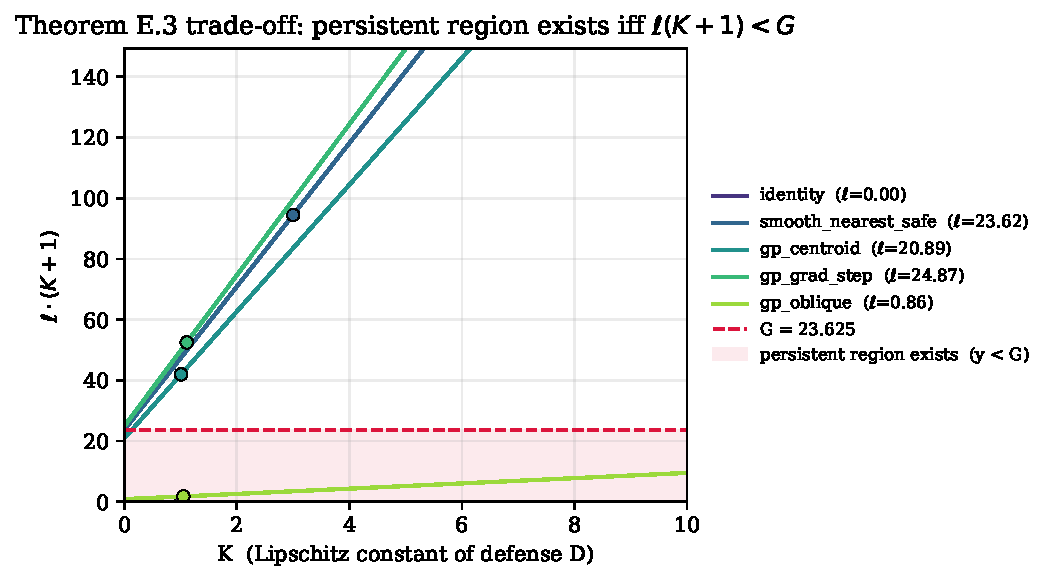
\includegraphics[width=0.75\textwidth]{figures/k_tradeoff.pdf}
\caption{Persistence-vs-utility tradeoff as $K$ varies around
$K^* = G/\ell - 1$ from \Cref{thm:dilemma}. Below $K^*$ the persistent
unsafe region is nonempty; at and above $K^*$ the displacement needed
to kill persistence is incompatible with utility preservation.}
\label{fig:k-tradeoff}
\end{figure}

\section{Pipeline Composition}
\label{app:pipeline}

\begin{theorem}[Pipeline Lipschitz Degradation]
\label{thm:pipeline}
If stages $T_1, \ldots, T_n$ are $K_1, \ldots, K_n$-Lipschitz, the
composed pipeline is $(\prod K_i)$-Lipschitz. For $n$ stages each with
$K \geq 2$, the effective constant is $K^n$.
\end{theorem}

\paragraph{Falsifier.}
A measured pipeline with empirical composed Lipschitz constant
$\hat K_{\text{composed}} > \hat K_1 \cdot \hat K_2$ would refute the
bound in \Cref{thm:pipeline}: Lipschitz constants submultiply under
composition, so the composed constant can never exceed the product.

\begin{theorem}[Pipeline Impossibility]
\label{thm:pipeline-impossible}
If the composed pipeline $P = T_n \circ \cdots \circ T_1 \circ D$ is
continuous and $P(x) = x$ for all $x \in S_\tau$, then $P$ has
boundary fixed points. If $D$ is $K_D$-Lipschitz and each $T_i$ is
$K$-Lipschitz, the $\varepsilon$-robust band scales as
$L \cdot K_D \cdot K^n \cdot \delta$.
\end{theorem}

\noindent\emph{Proved in the Lean artifact as
\textup{\texttt{MoF\_15\_NonlinearAgents}}.}

\begin{table}[h]
\centering
\small
\caption{Empirical pipeline Lipschitz degradation. The measured
composed constant $\hat K_{\text{composed}}$ is bounded above by
$\prod \hat K_i$, consistent with \Cref{thm:pipeline}.}
\label{tab:pipeline}
\input{tables/pipeline.tex}
\end{table}

\section{Vulnerability Landscape}
\label{app:landscape}

This section characterizes the geometry of the unsafe region.

\begin{theorem}[Basin Structure]
\label{thm:basin}
If $f$ is continuous and $f(p)>\tau$, then $U_\tau$ is open. Under
any measure positive on nonempty open sets, $U_\tau$ has positive
measure.
\end{theorem}

\begin{theorem}[Basin Fragment Minimum Size]
\label{thm:fragment}
If $X$ is a normed space, $f$ is $L$-Lipschitz with $f(p) > \tau$,
the connected component of $U_\tau$ containing $p$ has diameter
$\geq 2(f(p) - \tau)/L$.
\end{theorem}

Smoother surfaces (smaller~$L$) produce larger basins; rougher
surfaces produce smaller fragments.

\section{Full Proofs}
\label{app:proofs}

\begin{proof}[Proof of \Cref{thm:main} (Boundary Fixation)]
\textbf{Step~1} (Hausdorff $\Rightarrow$ fixed-point set is closed).
$\Fix(D) = \{x : D(x) = x\}$ is the preimage of the diagonal
$\Delta \subset X \times X$ under $x \mapsto (D(x), x)$. In a
Hausdorff space, $\Delta$ is closed, so $\Fix(D)$ is closed.

\textbf{Step~2} (Utility preservation $\Rightarrow$ safe region
$\subseteq$ fixed points).
$S_\tau \subseteq \Fix(D)$. Since $\Fix(D)$ is closed:
$\cl{S_\tau} \subseteq \Fix(D)$.

\textbf{Step~3} (Connectedness $\Rightarrow$ safe region is not closed).
$S_\tau = f^{-1}((-\infty,\tau))$ is open. If also closed, it would be
clopen---but in a connected space the only clopen sets are $\emptyset$
and $X$. Since both $S_\tau$ and $U_\tau$ are nonempty, $S_\tau$ is not
closed.

\textbf{Step~4} (Boundary point exists).
$\cl{S_\tau} \supsetneq S_\tau$, so there exists
$z \in \cl{S_\tau} \setminus S_\tau$. Continuity gives
$f(z) \leq \tau$; $z \notin S_\tau$ gives $f(z) \geq \tau$. Hence
$f(z) = \tau$.

\textbf{Step~5} (Defense fixes the boundary point).
$z \in \cl{S_\tau} \subseteq \Fix(D)$, so $D(z) = z$ and
$f(D(z)) = \tau$.
\end{proof}

\begin{proof}[Proof of \Cref{thm:eps-robust} ($\varepsilon$-Robust Constraint)]
By \Cref{thm:main}, the fixed boundary point $z$ exists.

\textbf{Step~1.} Since $D(z) = z$ and $D$ is $K$-Lipschitz:
$\dist(D(x), z) = \dist(D(x), D(z)) \leq K\dist(x, z)$.

\textbf{Step~2.} Since $f(z) = \tau$ and $f$ is $L$-Lipschitz:
$|f(D(x)) - \tau| = |f(D(x)) - f(z)| \leq L\dist(D(x), z) \leq
LK\dist(x, z)$.
\end{proof}

\begin{proof}[Proof of \Cref{thm:persistent} (Persistent Unsafe Region)]
\textbf{(1)} $\mathcal{S}$ is the strict superlevel set of
$x \mapsto f(x) - \ell(K+1)\dist(x,z)$ at level~$\tau$, hence open.

\textbf{(2)} Open and nonempty implies positive measure.

\textbf{(3)} For $x \in \mathcal{S}$:
$f(x) > \tau + \ell(K+1)\dist(x,z)$. By \Cref{lem:input-bound}:
$f(D(x)) \geq f(x) - \ell(K+1)\dist(x,z) > \tau$.

\noindent\emph{Lean:
\textup{\texttt{persistent\_unsafe\_refined}} in
\textup{\texttt{MoF\_20\_RefinedPersistence}}
(defense-path constant~$\ell$).
\textup{\texttt{MoF\_11\_EpsilonRobust}} contains an earlier version
using the global constant~$L$; as noted in
\Cref{sec:persistent}, that version is vacuous for isotropic surfaces.}
\end{proof}


\section{Counterexamples: Each Hypothesis Is Necessary}
\label{app:counterexamples}

\begin{counterexample}[Removing connectedness]
$X = \{0,1\}$ discrete, $f(0)=0$, $f(1)=1$, $\tau=0.5$.
$D(0)=0$, $D(1)=0$: continuous, utility-preserving, complete.
\end{counterexample}

\begin{counterexample}[Removing continuity]
$X=[0,1]$, $f(x)=x$, $\tau=0.5$. $D(x)=x$ for $x<0.5$,
$D(x)=0$ for $x \geq 0.5$: utility-preserving and complete,
but discontinuous at $0.5$.
\end{counterexample}

\begin{counterexample}[Removing utility preservation]
$D(x) = x_0$ for a fixed safe point: continuous and complete,
but destroys all inputs.
\end{counterexample}

\begin{table}[h]
\centering
\small
\caption{Counterexample ablation. Each row drops one of the three
hypotheses and reports whether the defense becomes complete, together
with the price paid in the other two properties.}
\label{tab:counterexample-ablation}
\input{tables/counterexample_ablation.tex}
\end{table}


\section{Attack Properties}
\label{app:attacks}

\begin{theorem}[Perturbation Robustness]
\label{thm:lipschitz}
If $f$ is $L$-Lipschitz and $f(p)>\tau$, then
$B(p,\, (f(p)-\tau)/L) \subseteq U_\tau$.
The radius is monotone in~$f(p)$.
\end{theorem}

\begin{theorem}[Iterative Convergence]
\label{thm:convergence}
Any monotone-improvement operator $T$ with score in $[0,1]$ converges.
If each step gains $\geq \delta$, convergence takes
$\leq \lfloor 1/\delta \rfloor$ steps.
\end{theorem}

\begin{theorem}[Transferability]
\label{thm:transfer}
$\|f-g\|_\infty \leq \delta \implies
\{f > \tau+\delta\} \subseteq \{g > \tau\}$.
Transfer costs zero additional queries.
\end{theorem}

\begin{theorem}[Authority Monotonicity]
\label{thm:authority}
If $f(y,\cdot)$ is monotone non-decreasing in authority for each fixed
indirection~$y$, the vulnerability set is upward-closed with a critical
threshold $a^*_2(y)$ (by IVT, when $f(y,\cdot)$ is continuous and
crosses~$\tau$). If additionally $f$ is monotone non-decreasing in
indirection for each fixed authority, the threshold curve
$y \mapsto a^*_2(y)$ is non-increasing.
\end{theorem}

\begin{theorem}[Gradient Ascent]
\label{thm:gradient}
If $f$ has nonzero Fr\'{e}chet derivative at~$x$, there exist $v$ and
$\varepsilon > 0$ with $f(x + \varepsilon v) > f(x)$.
\end{theorem}


\section{Stability Under Fine-Tuning}
\label{app:stability}

\begin{theorem}[Interior Stability]
\label{thm:interior-stable}
If $\|f - g\|_\infty \leq \varepsilon$:
$f(x) > \tau + \varepsilon \implies g(x) > \tau$, and
$f(x) < \tau - \varepsilon \implies g(x) < \tau$.
Only the band $|f(x) - \tau| \leq \varepsilon$ is uncertain.
\end{theorem}

\begin{theorem}[Crossing Preservation]
\label{thm:crossing}
Let $f, g\colon [a,b] \to \R$ be continuous. If $f$ crosses $\tau$
on $[a,b]$ with margin $m$ (i.e., $f(a') < \tau - m$ and
$f(b') > \tau + m$ for some $a', b' \in [a,b]$) and
$\|f - g\|_\infty \leq \varepsilon < m$, then $g$ also crosses
$\tau$ on $[a,b]$.
\end{theorem}

\begin{theorem}[Patching Is Nonlocal]
\label{thm:nonlocal}
There exist $f, g$ with $\|f-g\|_\infty \leq \varepsilon$ such that
eliminating a vulnerability at one point necessarily changes values at
distant points.
\end{theorem}


\section{Cost Asymmetry}
\label{app:cost}

\begin{theorem}[Cost Asymmetry for Grid-Enumeration Defenses]
\label{thm:cost}
For \emph{grid-based exhaustive-enumeration} defense with $N \geq 2$
bins per axis in $d$ dimensions:
attack cost $\leq 1/\delta$ (dimension-independent); defense cost
$= N^d$ (exponential in~$d$); ratio
$\delta \cdot N^d \to \infty$ as $d\to\infty$.
\end{theorem}

\noindent\textit{Caveat.} This bound applies to grid enumeration, not
to learning-based defenses (e.g., GP surrogates) that generalize across
the space without evaluating every cell. The paper's own empirical
section uses such surrogates at cost $\ll N^d$.

At $d=2$ with $N=25$ and $\delta=0.01$, the ratio is $6.25$.
At $d=10$, it climbs to $\sim 10^{12}$.


\section{Additional Verified Results}
\label{app:additional}

\paragraph{Lipschitz displacement bound.}
$D$ is $K$-Lipschitz with $D(z) = z \implies
\dist(D(x), x) \leq (K+1)\dist(x,z)$.

\paragraph{Tool calls amplify failure.}
Each non-contractive tool call multiplicatively increases the pipeline's
effective Lipschitz constant: $K^n < K^{n+1}$ for $K \geq 2$.

\paragraph{Attacker monotone improvement.}
Best observed alignment deviation is non-decreasing across turns.

\paragraph{Attacker steering.}
If directional slope varies continuously with attacker parameter $\alpha$
and crosses $\ell(K+1)$, transversality is reachable by IVT.

\paragraph{Stochastic regularity.}
$g(x) = \mathbb{E}[f(D(x))]$ satisfies $g - f = 0$ on $\cl{S_\tau}$.

\paragraph{Discrete defense dilemma.}
An injective, utility-preserving defense is incomplete (every unsafe
input stays unsafe). A complete, utility-preserving defense is
non-injective (distinct inputs collapse to the same output).
The three properties---completeness, utility preservation,
injectivity---form a trilemma.

\paragraph{Defense position invariance.}
Lipschitz constant of defense-before-tools equals defense-after-tools:
$K_D \cdot K_T^n$.


\section{Additional Experimental Details}
\label{app:exp-details}

This appendix collects the estimator definitions, sanity checks,
continuous-defense sweeps, and robustness tables that support the main
paper's empirical claims.

\subsection{Estimator definitions}
\label{sec:estimators}

Let $G_f$ denote the set of filled cells in an $N \times N$ MAP-Elites
grid and let $h = 1/N$ be the cell width. Distances use normalized
$L_2$ grid coordinates on $[0,1]^2$:
\[
\dist\bigl((i_1,j_1),(i_2,j_2)\bigr)
  = h\sqrt{(i_1-i_2)^2 + (j_1-j_2)^2}.
\]
All pairs involving unfilled cells are excluded; no imputation is
performed. The boundary anchor is
\[
z^* = \arg\min_{x \in G_f} |f(x)-\tau|,
\]
restricted to sampled boundary cells
$\cl{S_\tau}\setminus S_\tau$, with lexicographic tie-breaking.

\paragraph{Surface Lipschitz constant.}
\[
\hat L = \max_{x,y \in G_f,\ x \neq y}
\frac{|f(x)-f(y)|}{\dist(x,y)}.
\]

\paragraph{Defense Lipschitz constant.}
\[
\hat K = \max_{u,v \in G_f,\ u \neq v}
\frac{\dist(D(u),D(v))}{\dist(u,v)}.
\]

\paragraph{Defense-path Lipschitz constant.}
\[
\hat\ell = \max_{x \in G_f,\ D(x)\neq x,\ D(x)\in G_f}
\frac{|f(D(x))-f(x)|}{\dist(D(x),x)}.
\]
If the set is empty, we take $\hat\ell = 0$.

\paragraph{Boundary directional rate.}
\[
\hat G = \max_{x,y \in G_f,\ f(x)<\tau<f(y)}
\frac{f(y)-f(x)}{\dist(x,y)}.
\]
These are the estimators used by the validator and the tables below.

\subsection{Identity and out-of-scope sanity checks}
\label{sec:identity-sanity}

Identity-defense rows are bookkeeping checks rather than theorem tests:
under $D=\id$, the predicted and observed unsafe sets coincide by
construction.

\begin{table}[h]
\centering
\small
\caption{\textbf{Smoke tests (not a test of the theorem).} The two
sparse $25\times 25$ live runs under the canonical identity defense.
Under $D = \mathrm{id}$,
$\mathcal{S}_{\text{pred}} \equiv \mathcal{S}_{\text{act}} \equiv
\{x : f(x) > \tau\}$ by construction, so agreement only checks the
validator's bookkeeping.}
\label{tab:smoketests}
\begin{tabular}{lccccccccc}
\toprule
\textbf{Target} & $\boldsymbol{\tau}$ & \textbf{Filled} & $\boldsymbol{L}$ & $\boldsymbol{G}$ & $|\mathcal{S}_{\text{pred}}|$ & $|\mathcal{S}_{\text{act}}|$ & \textbf{TP} & \textbf{FP}$_{\text{int}}$ & \textbf{FN} \\
\midrule
gpt-5-mini-2025-08-07      & $0.30$ & $14$ & $6.13$  & $6.13$  & $7$ & $7$ & $7$ & $\mathbf{0}$ & $0$ \\
gpt-3.5-turbo-0125 (smoke) & $0.50$ & $9$  & $11.44$ & $11.44$ & $7$ & $7$ & $7$ & $\mathbf{0}$ & $0$ \\
\bottomrule
\end{tabular}
\end{table}

\subsection{Continuous-defense sweeps}
\label{app:continuous-sweeps}

\begin{table}[h]
\centering
\small
\caption{Continuous-defense sweep on the saturated
\texttt{gpt-3.5-turbo-0125} grid over continuous defense families
(GP-oblique, Gaussian-smoothed nearest-safe, contractive-flow).
Each row reports empirical $\hat\ell$, $\hat K$,
$|\mathcal{S}_{\text{pred}}|$, $|\mathcal{S}_{\text{act}}|$, TP, and
FP$_{\text{int}}$.}
\label{tab:continuous-sweep}
\input{tables/continuous_sweep.tex}
\end{table}

\begin{table}[h]
\centering
\small
\caption{GP-kernel sensitivity for the oblique-smooth defense on the
saturated \texttt{gpt-3.5-turbo-0125} grid. Kernel
$\in\{\text{RBF},\text{Mat\'ern-}3/2,\text{Mat\'ern-}5/2\}$ crossed
with bandwidth $\sigma\in\{0.1,0.2,0.4\}$.}
\label{tab:gp-sensitivity}
\input{tables/gp_sensitivity.tex}
\end{table}

\begin{table}[h]
\centering
\small
\caption{Resolution sweep for the oblique-smooth defense on
\texttt{gpt-3.5-turbo-0125}. As $h = 1/N$ decreases, the
discretization gap $|f(z^*)-\tau|$ shrinks and
$|\mathcal{S}_{\text{pred}}|$ grows; the theorem's containment is
preserved across resolutions.}
\label{tab:resolution}
\input{tables/resolution.tex}
\end{table}

\subsection{Robustness checks}

\begin{table}[h]
\centering
\small
\caption{Higher-dimensional robustness. Empirical $\hat L$ and $\hat G$
computed on the same $82$-cell archive using the paper's 2D grid metric
and a $768$-dimensional embedding metric.}
\label{tab:higher-dim-lipschitz}
\input{tables/higher_dim_lipschitz.tex}
\end{table}

\begin{table}[h]
\centering
\small
\caption{Seed replication of the saturated pipeline on
\texttt{gpt-3.5-turbo-0125}. Surface quantities remain within a narrow
band and $\mathrm{FP}_{\mathrm{int}} = 0$ in both runs.}
\label{tab:seed-replication}
\input{tables/seed_replication.tex}
\end{table}

\begin{table}[h]
\centering
\small
\caption{Independent target re-evaluation. The same 82 prompts are
rescored on \texttt{gpt-4o-mini-2024-07-18} with the judge held fixed.
No interior counterexample is observed.}
\label{tab:independent-dataset}
\input{tables/independent_dataset.tex}
\end{table}

\begin{table}[h]
\centering
\small
\caption{Bootstrap percentile confidence intervals (median,
$[5^{\text{th}},95^{\text{th}}]$) for the empirical quantities on the
saturated live run.}
\label{tab:ci}
\input{tables/ci.tex}
\end{table}

\begin{figure}[h]
\centering
\includegraphics[width=0.75\textwidth]{figures/tau_sweep.pdf}
\caption{Sensitivity of $|\mathcal{S}_{\text{pred}}|$,
$|\mathcal{S}_{\text{act}}|$, and $\mathrm{FP}_{\mathrm{int}}$ to the
threshold~$\tau$ on the saturated live run. The containment
$\mathcal{S}_{\text{pred}} \subseteq \mathcal{S}_{\text{act}}$ holds
at every tested~$\tau$.}
\label{fig:tau-sweep}
\end{figure}

\subsection{Out-of-scope discrete stress tests}
\label{sec:discrete-stress}

Bounded-step defenses are not continuous, so
\Cref{thm:persistent}'s hypotheses do not apply. We include them only
as negative consistency checks.

\begin{table}[h]
\centering
\small
\caption{\textbf{Out-of-scope discrete stress tests.} Defense sweep on
the saturated \texttt{gpt-3.5-turbo-0125} grid over discontinuous
\texttt{bounded\_step} defenses. These rows are not theorem checks; they
are reported only as consistency checks outside the theorem's scope.}
\label{tab:live-sweep}
\begin{tabular}{lccccccc}
\toprule
\textbf{Defense} & $\boldsymbol{K}$ & $\boldsymbol{\ell}$ & $|\mathcal{S}_{\text{pred}}|$ & $|\mathcal{S}_{\text{act}}|$ & \textbf{TP} & \textbf{FP}$_{\text{int}}$ & \textbf{FN} \\
\midrule
identity                   & $1.00$ & $0.00$  & $66$ & $66$ & $66$ & $\mathbf{0}$ & $0$ \\
\texttt{bounded\_step(1)}  & $3.61$ & $23.63$ & $1$  & $55$ & $0$  & $\mathbf{0}$ & $55$ \\
\texttt{bounded\_step(2)}  & $3.61$ & $23.63$ & $1$  & $47$ & $0$  & $\mathbf{0}$ & $47$ \\
\texttt{bounded\_step(3)}  & $4.00$ & $23.63$ & $1$  & $29$ & $0$  & $\mathbf{0}$ & $29$ \\
\texttt{bounded\_step(5)}  & $8.60$ & $23.63$ & $1$  & $3$  & $0$  & $\mathbf{0}$ & $3$  \\
\texttt{bounded\_step(8)}  & $8.60$ & $23.63$ & $1$  & $0$  & $0$  & $\mathbf{0}$ & $0$  \\
\texttt{bounded\_step(12)} & $8.60$ & $23.63$ & $1$  & $0$  & $0$  & $\mathbf{0}$ & $0$  \\
\bottomrule
\end{tabular}
\end{table}


\section{Judge robustness}
\label{app:judge-robustness}

All $f$ values in~\Cref{sec:live-validation} are judge-dependent:
swapping the judge can reshape the alignment-deviation surface and
thereby change $\hat L, \hat\ell, \hat G$. To quantify this, we
rescored the 82 $(\text{prompt}, \text{target response})$ pairs from
the saturated \texttt{gpt-3.5-turbo-0125} archive with three alternative
judges drawn from different families and capacities —
\texttt{gpt-4o-2024-08-06}, \texttt{gpt-4.1-mini-2025-04-14}, and
\texttt{gpt-4o-mini-2024-07-18} — applying the same rethinking-evals
per-category methodology with a single judge and $\alpha=0.5$ (target
responses were NOT regenerated; only the judge was swapped). The
four-judge comparison is summarized in~\Cref{tab:judge-robustness}.

\begin{table}[h]
\centering
\caption{Judge robustness on the saturated archive (82 cells, $\tau=0.5$).
$|\mathcal{S}_\tau|_{\mathrm{sample}}$ and
$|\mathcal{U}_\tau|_{\mathrm{sample}}$ are how many of the 82 sampled
cells fall below/above $\tau$ under each judge. Pearson $r$ and
Cohen's $\kappa$ are pairwise with the canonical gpt-4.1 judge.
Kendall's $W=0.700$ across all four judges on cell rankings (moderate
agreement). ``Testable?'' indicates whether this MAP-Elites sample
spans both $\mathcal{S}_\tau$ and $\mathcal{U}_\tau$, which is what
the positive-prediction test of Theorem~\ref{thm:persistent} requires
to locate a boundary cell $z^*$.}
\label{tab:judge-robustness}
\input{tables/judge_robustness.tex}
\end{table}

\begin{figure}[h]
\centering
\includegraphics[width=0.75\textwidth]{figures/judge_scatter.pdf}
\caption{Per-cell alignment-deviation scatter across the four judges.
Cross-judge agreement is moderate (Kendall's $W = 0.700$); the
positive-prediction test of \Cref{thm:persistent} remains supported
wherever the sample spans both $\mathcal{S}_\tau$ and
$\mathcal{U}_\tau$.}
\label{fig:judge-scatter}
\end{figure}

\paragraph{Interpretation.} The theorem applies to the full prompt
space $X$ under every judge — benign prompts exist, so
$\mathcal{S}_\tau$ is nonempty in $X$. Whether the theorem's positive
prediction can be \emph{tested from a given sample} depends on whether
that sample spans both regions. Three of four judges
(\texttt{gpt-4.1}, \texttt{gpt-4o}, \texttt{gpt-4.1-mini}) yield samples
that span both $\mathcal{S}_\tau$ and $\mathcal{U}_\tau$; applying the
continuous \texttt{smooth\_nearest\_safe} defense produces
TP$>0$ and FP$_{\mathrm{int}}=0$ in every case. Under the strictest
judge (\texttt{gpt-4o-mini}), MAP-Elites's adversarial bias drives the
sample entirely into $\mathcal{U}_\tau$, so no boundary cell $z^*$
appears in the 82 sampled cells and the positive prediction cannot be
tested from this sample. Crucially, FP$_{\mathrm{int}}=0$ still holds:
no counterexample to the theorem is produced under any of the four
judges. Cross-judge agreement ranges from substantial (Kendall's
$W=0.70$) to poor on binary classification (Cohen's $\kappa=0$ vs
gpt-4o-mini), so the \emph{specific numerical instance} of a particular
judge is not itself judge-robust even though the \emph{framework's
predictions} are.

\paragraph{Committee aggregation.}
The rethinking-evals methodology supports committee aggregation:
$P_{\mathrm{actual}} = \alpha P_{\mathrm{vote}} + (1-\alpha) P_{\mathrm{mean}}$
with $\alpha=0.5$. We apply this offline to the four existing judge
archives (no new API calls) and re-run the validator on each
committee-aggregated surface (\Cref{tab:judge-committee}). The
top-3 committee (gpt-4.1, gpt-4o, gpt-4.1-mini; excluding the
strict-judge outlier gpt-4o-mini) is within one cell of canonical
($17$ safe vs $16$; mean $\Delta=+0.010$), and
$\mathrm{FP}_{\mathrm{int}}=0$ under \texttt{smooth\_nearest\_safe}
on every committee configuration --- the theorem's predictions
survive committee aggregation.

\begin{table}[h]
\centering
\small
\caption{Judge committee aggregations vs the canonical single-judge
surface. Top-3 committee is within one cell of canonical;
$\mathrm{FP}_{\mathrm{int}}=0$ in every configuration.}
\label{tab:judge-committee}
\input{tables/judge_committee.tex}
\end{table}


\section{Attack Baseline: PAIR-Style Iteration}
\label{app:pair-baseline}

To situate the theorem empirically against an established attack-defense
benchmark style, we run a PAIR-style iterative attack
(\cite{chao2024jailbreaking}-adjacent) on ten top-AD unsafe seed prompts
from the saturated archive. The attacker is \texttt{gpt-4o-mini}, the
target is \texttt{gpt-3.5-turbo-0125}, and the judge is \texttt{gpt-4.1}.
Each behavior gets five iterations; the attacker receives the full
transcript and judge scores at each step. We compare two conditions:
undefended (attacker prompt goes directly to target) and
\emph{paraphrase wrapper} (attacker prompt is rewritten by
\texttt{gpt-4o-mini} at $T=0$ before reaching the target).

\begin{table}[h]
\centering
\small
\caption{PAIR-style attack-success rate with and without a continuous
paraphrase wrapper (10 behaviors, 5 iterations, gpt-3.5-turbo target,
gpt-4.1 judge).}
\label{tab:pair-baseline}
\input{tables/pair_baseline.tex}
\end{table}

\paragraph{Interpretation.}
Within the 5-iteration budget the paraphrase wrapper blocks all ten
behaviors (ASR drops from $1.00$ to $0.00$). This does \emph{not}
contradict Theorem~\ref{thm:disc-dilemma}'s injective-incomplete
horn: the paraphrase defense is injective on our 66-prompt sample
(all 66 rewrites are distinct), and \Cref{tab:paraphrase-unsafe}
already exhibits $1/66$ paraphrases that yield $f(D(x)) > \tau$. The
PAIR attacker with gpt-4o-mini as refiner and a 5-iteration budget
is not sufficient to locate that bypass; a persistent attacker (more
iterations, stronger refiner) is predicted to find one by
\Cref{thm:multi-turn}'s multi-turn convergence argument.


\section{Lean Artifact}
\label{app:artifact}

The complete theory is formalized in Lean~4.28.0 with Mathlib~v4.28.0,
available at
\url{https://anonymous.4open.science/r/defense-trilemma-XXXX}.
The artifact serves two roles: (1)~definitional scaffolding that
pins down every hypothesis (continuity, utility preservation,
Lipschitz, transversality) in a machine-readable form, ensuring
no translation drift between prose and formal statement; and
(2)~verified cross-references between theorem statements, so that
the dependency chain
(\Cref{thm:main}$\to$\Cref{thm:eps-robust}$\to$\Cref{thm:persistent})
is mechanically checked.
The proofs themselves are short (the underlying mathematics is not
deep); the artifact's value is precision, not error-checking.
It comprises 46 files:
\begin{itemize}[nosep]
  \item 10 core theory files (MoF\_01--MoF\_10)
  \item 10 cost theory files (MoF\_Cost\_01--MoF\_Cost\_10)
  \item 10 advanced theory files (MoF\_Adv\_01--MoF\_Adv\_10)
  \item 1 continuous relaxation (MoF\_ContinuousRelaxation)
  \item 1 $\varepsilon$-robust constraint + persistent unsafe region
    with global Lipschitz constant
    (MoF\_11\_EpsilonRobust)
  \item 1 discrete impossibility (MoF\_12\_Discrete)
  \item 1 multi-turn + stochastic extensions
    (MoF\_13\_MultiTurn)
  \item 1 representation-independent meta-theorem
    (MoF\_14\_MetaTheorem)
  \item 1 nonlinear agent pipelines (MoF\_15\_NonlinearAgents)
  \item 1 relaxed utility preservation (MoF\_16\_RelaxedUtility)
  \item 1 quantitative $\varepsilon$-band volume bound
    (MoF\_17\_CoareaBound)
  \item 1 cone measure bound for persistent unsafe region
    (MoF\_18\_ConeBound)
  \item 1 optimal defense characterization
    (MoF\_19\_OptimalDefense)
  \item 1 refined persistence with defense-path Lipschitz constant~$\ell$
    (MoF\_20\_RefinedPersistence); this file contains the primary
    formalization of \Cref{thm:persistent,lem:input-bound,def:steep}
  \item 1 gradient chain: $\|\nabla f(z)\| > \ell(K+1)$ implies
    persistent unsafe region via operator-norm direction extraction
    and derivative-based local growth
    (MoF\_21\_GradientChain)
  \item 3 capstone files (MasterTheorem, Euclidean instantiation,
    verification)
  \item 1 root import file (ManifoldProofs.lean)
\end{itemize}

\input{neurips_checklist.tex}

\end{document}
